\documentclass{article}
\usepackage[utf8]{inputenc}
\usepackage{mathtools}
\usepackage{pgfplots}
\usepackage{natbib}
\usepackage{amsmath}
\usepackage{amssymb}
\usepackage{amsfonts}
\usepackage{natbib}
\usepackage{graphicx}
\usepackage{minted}
\usepackage{ dsfont }
\usepackage{xcolor}
\usepackage{adjustbox}
\usepackage{soul}


\usepackage[a4paper,margin=1in,footskip=0.25in]{geometry}
\allowdisplaybreaks


\title{CSE546 Machine Learning HW3}
\author{Bobby Deng | 1663039 | dengy7 }
\date{16 May 2020}

\begin{document}
\maketitle


\section*{A.1}
\subsection*{a. [2 points] True or False: Given a data matrix $X \in R^{n \times d }$ where d is much smaller than n, if we project our data onto a k dimensional subspace using PCA where k = rank(X), our projection will have 0 reconstruction error (we find a perfect representation of our data, with no information loss).}

\fcolorbox{red}{white}{ Solution:} \\
True: If k is rank(k), it means we have captured all variation from the data, and it can perfectly represent the data.

\subsection*{b. [2 points] True or False: The maximum margin decision boundaries that support vector machines construct have the lowest generalization error among all linear classifiers.}
\fcolorbox{red}{white}{ Solution:} \\
False, SVM gives us a nice result, but it is not necessarily the lowest. It really depends on use cases and datasets. For example, the underlining true model need to be considered as well.

\subsection*{c. [2 points] True or False: An individual observation xi can occur multiple times in a single bootstrap sample from a dataset X, even if xi only occurs once in X.}
\fcolorbox{red}{white}{ Solution:} \\
True: Bootstrap is done by draw sample with replacement.

\subsection*{d. [2 points] True or False: Suppose that the SVD of a square $n \times n$ matrix X is $USV^T$, where S is a diagonal $n \times n$ matrix. Then the rows of V are equal to the eigenvectors of $X^TX$.}
\fcolorbox{red}{white}{ Solution:} \\
False, the columns are eigenvectors.

\subsection*{e. [2 points] True or False: Performing PCA to reduce the feature dimensionality and then applying the Lasso results in an interpretable linear model.}
\fcolorbox{red}{white}{ Solution:} \\
False: When we use PCA, the data lost the interpretability, the data are reconstructed. Lasso can not make this model interpret-able.

\subsection*{f. [2 points] True or False: choosing k to minimize the k-means objective (see Equation (1) below) is a good way to find meaningful clusters.}
\fcolorbox{red}{white}{ Solution:} \\
False, the bigger k we used, the less distance we will have, and this does not mean that our model gets better and better. 

\subsection*{g. [2 points] Say you trained an SVM classifier with an RBF kernel $ K(u, v) = exp( - \frac{||u-v||^2_2}{ 2\sigma^2 } ) $. It seems to under-fit the training set: should you increase or decrease $ \sigma$?}
\fcolorbox{red}{white}{ Solution:} \\
We should decrease $\sigma$ to increase some complexity of our model. When $\sigma$ is big, the boundary tends to be pretty smooth, but when $\sigma$ getting smaller, the boundary gets more strict.



\section*{A.2}
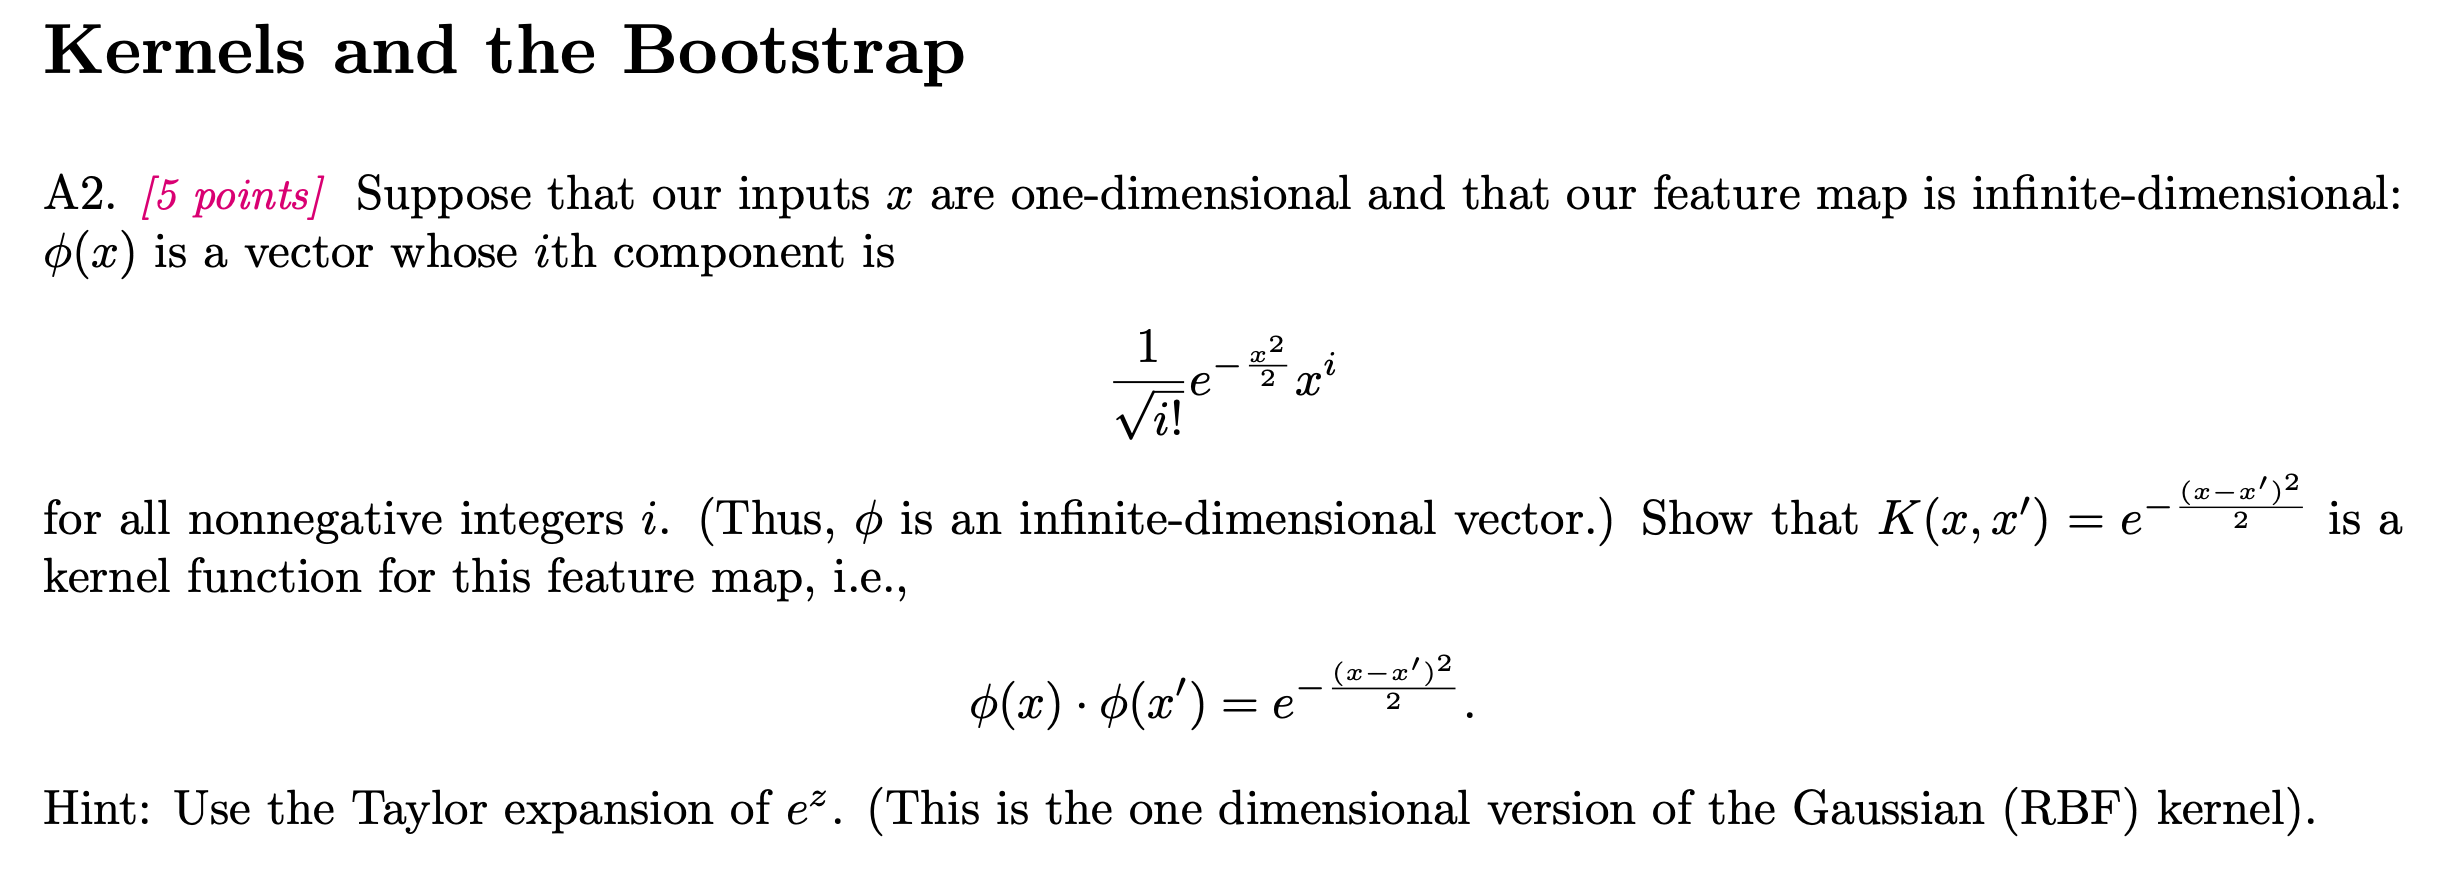
\includegraphics[width=16cm]{img/A2.png}

\fcolorbox{red}{white}{ Solution:} \\

From the question, we know that:
\[ K(x,x') = \phi(x) \cdot \phi(x') \]
We also can get that:
\[ \phi(x) = \frac{1}{\sqrt{i!}} e^{\frac{-x^2}{2}} x^i \]
\[ \phi(x') =  \frac{1}{\sqrt{i!}} e^{-\frac{1}{2}} * 1 = \frac{1}{\sqrt{i!}} \frac{1}{\sqrt{e}} \]
Then do the dot product:
\[ K(x,x') = \phi(x) \cdot \phi(x') \]
\[ \phi(x) \cdot \phi(x') = \sum_{i=0}^{\infty} \frac{1}{\sqrt{i!}} e^{\frac{-x^2}{2}} x^1  \frac{1}{\sqrt{i!}} \frac{1}{\sqrt{e}}  \]

\[ \phi(x) \cdot \phi(x') = \sum_{i=0}^{\infty}  \frac{1}{i!} e^{\frac{-x^2}{2}} x^i \frac{1}{\sqrt{e}} \]

\[ \phi(x) \cdot \phi(x') = \sum_{i=0}^{\infty}  \frac{1}{i!} e^{ - \frac{x^2 + 1}{2}} x^i \]

\[ \phi(x) \cdot \phi(x') = e^{ - \frac{x^2 + 1}{2}} \sum_{i=0}^{\infty}  \frac{x^i}{i!} \]

After doing Taylor Expansion:
\[ \phi(x) \cdot \phi(x') = e^{ - \frac{x^2 + 1}{2}} e^x \]
\[ \phi(x) \cdot \phi(x') = e^{ - \frac{x^2 - 2x + 1}{2}} \]
\[ \phi(x) \cdot \phi(x') = e^{ - \frac{(x-1)^2}{2}} \]

Here we know that $x' = 1$, then:
\[ \phi(x) \cdot \phi(x') = e^{ - \frac{(x-x')^2}{2}} \]
So, 
\[ K(x, x') = e^{ - \frac{(x-x')^2}{2}} \]

\section*{A.3}

\subsection*{a.}
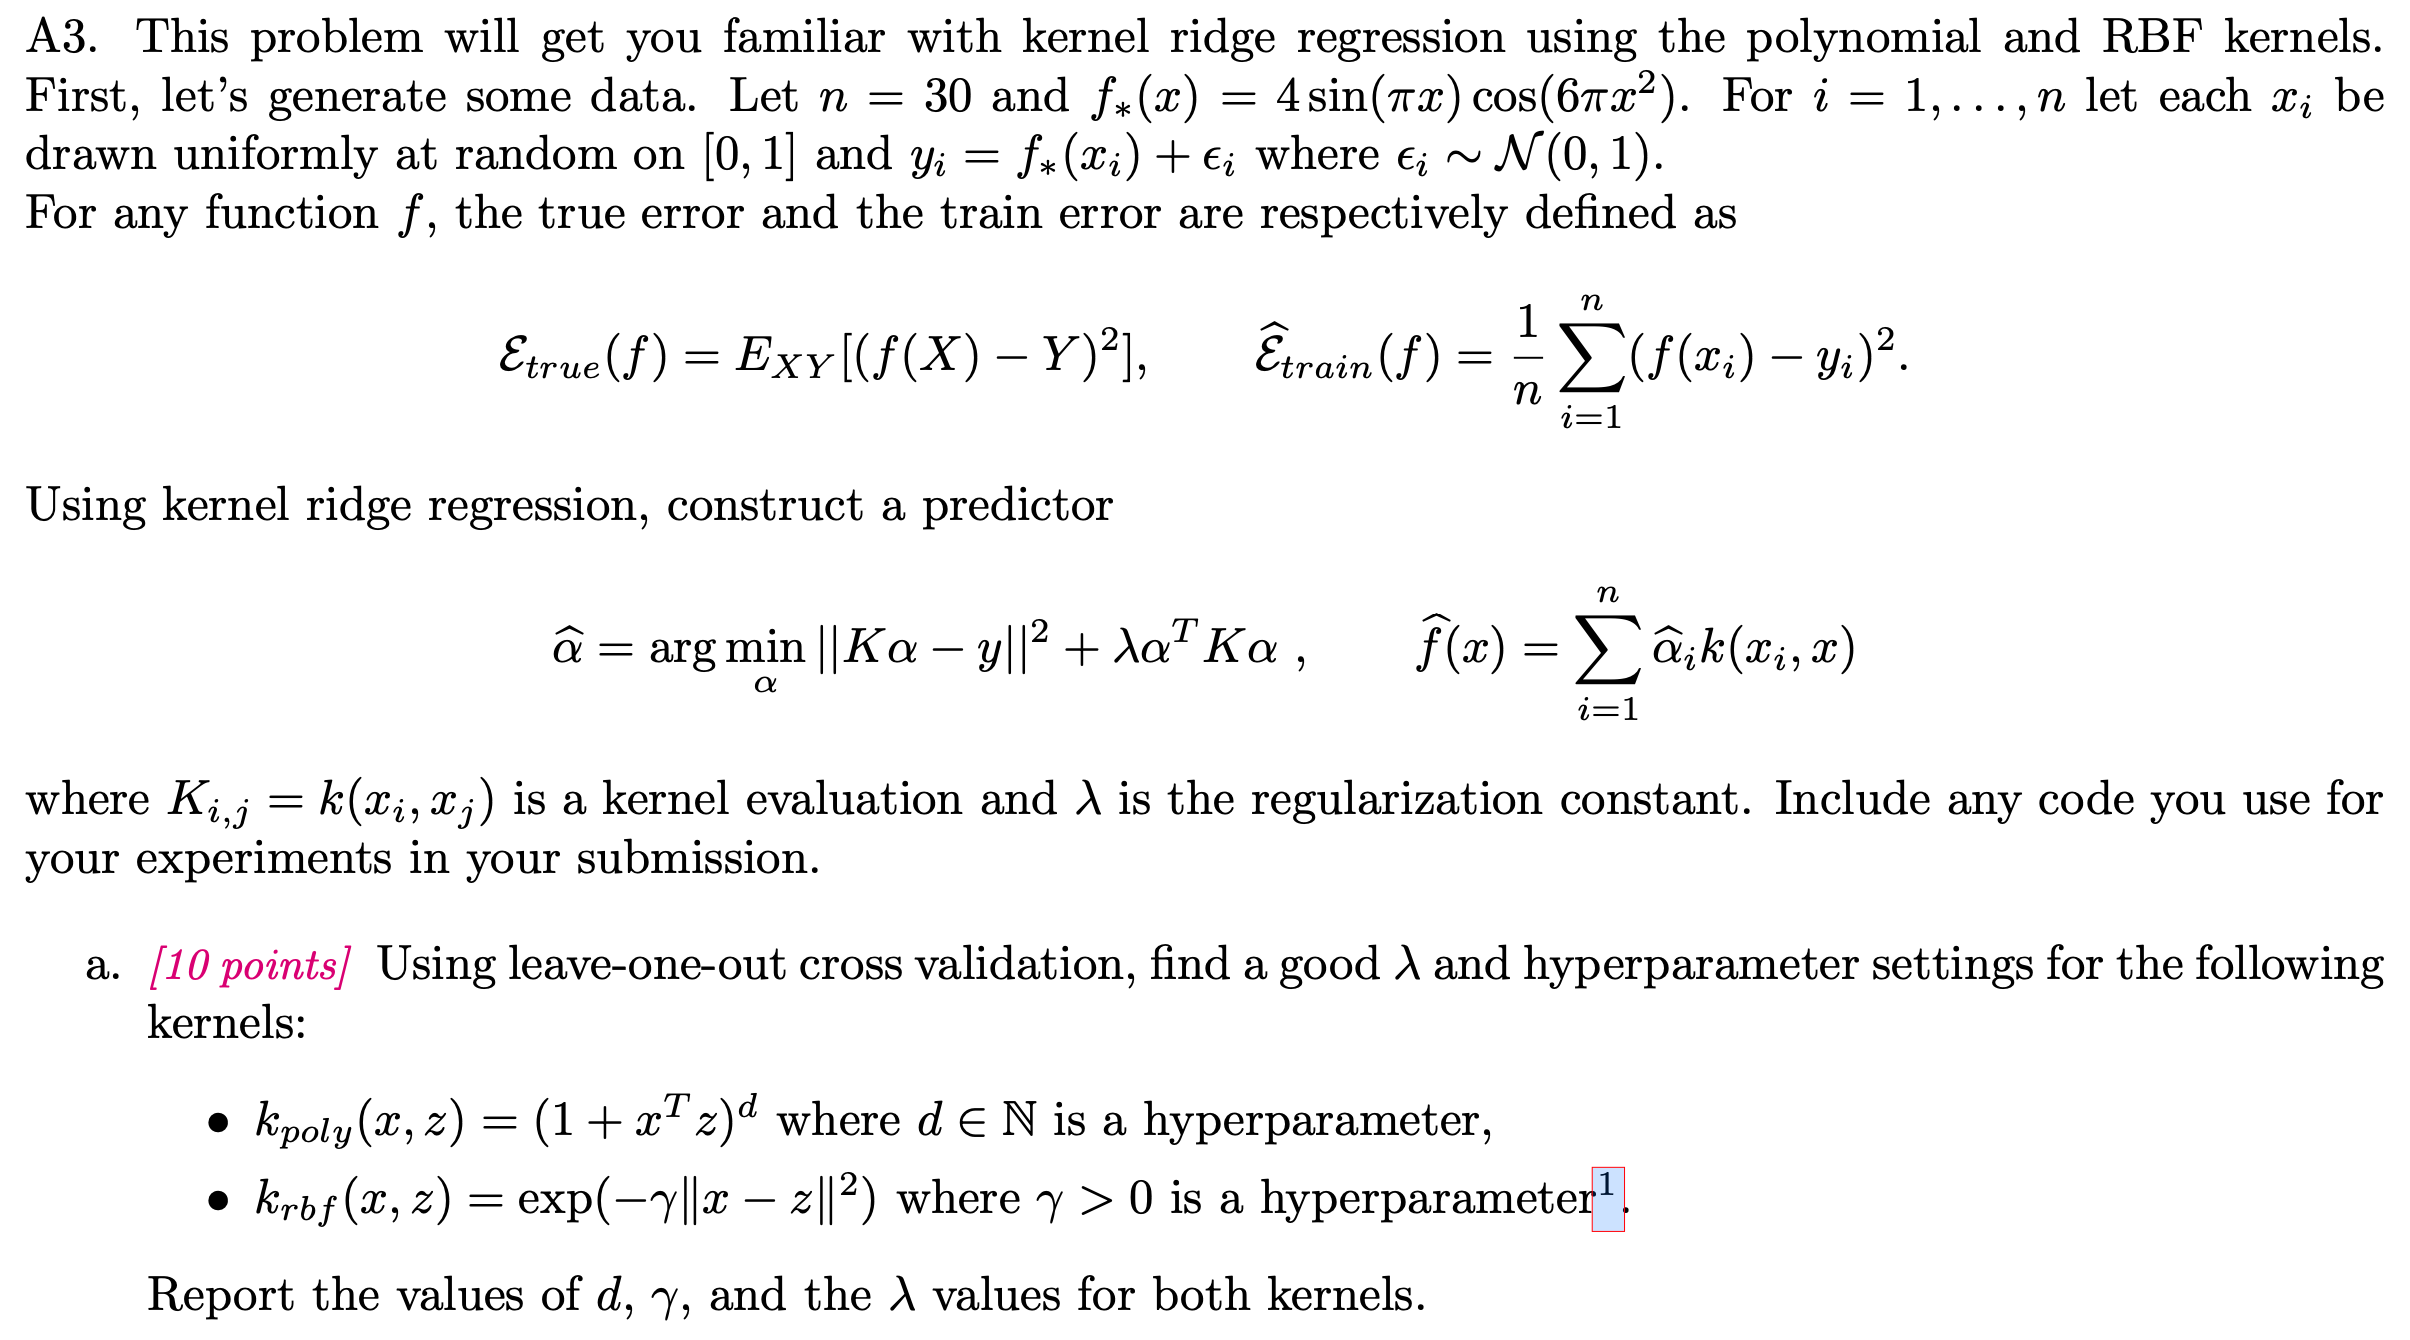
\includegraphics[width=16cm]{img/A3a.png}
\fcolorbox{red}{white}{ Solution:}

Best lamb for Poly kernel:  0.48828125. \newline
Best d for Poly kernel:  44. \newline

Best gamma for RBF kernel is :  8.175399541327897 \newline
Best Lambda for RBF kernel is : 9.313225746154785e-07



\subsection*{b.}
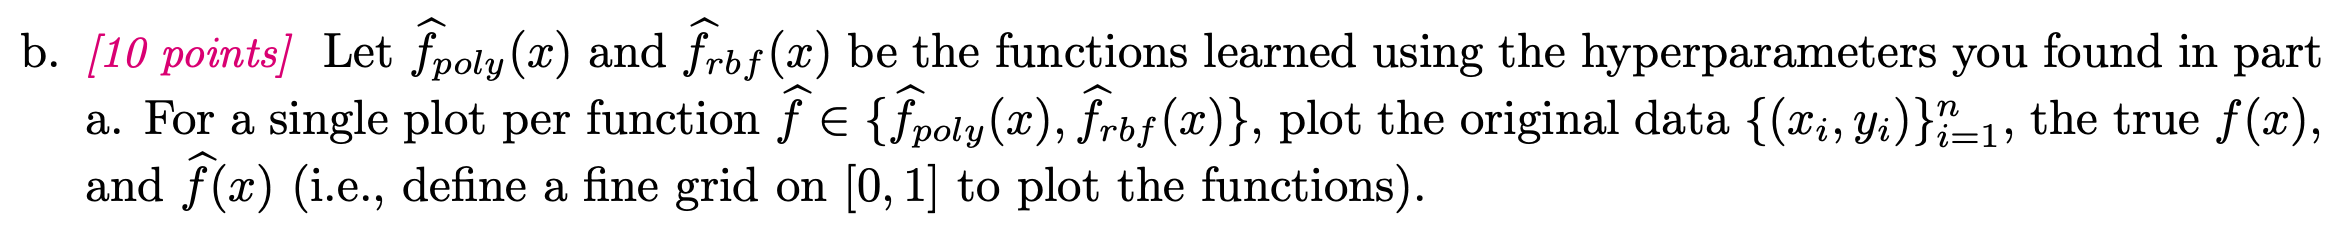
\includegraphics[width=16cm]{img/A3b.png}
\fcolorbox{red}{white}{ Solution:}

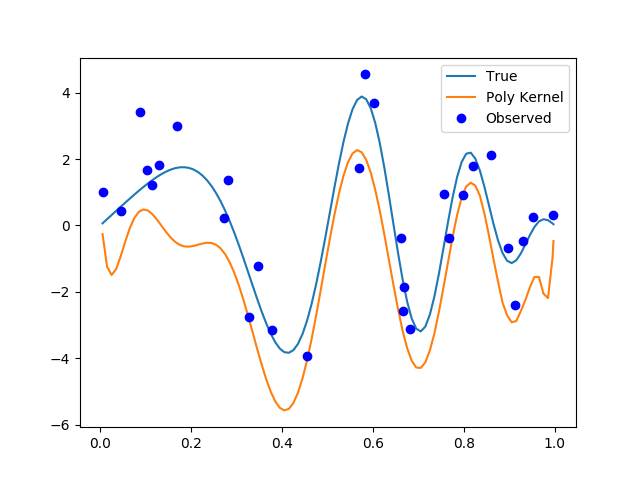
\includegraphics[width=9cm, height=6cm]{plots/A3b_1.png} 
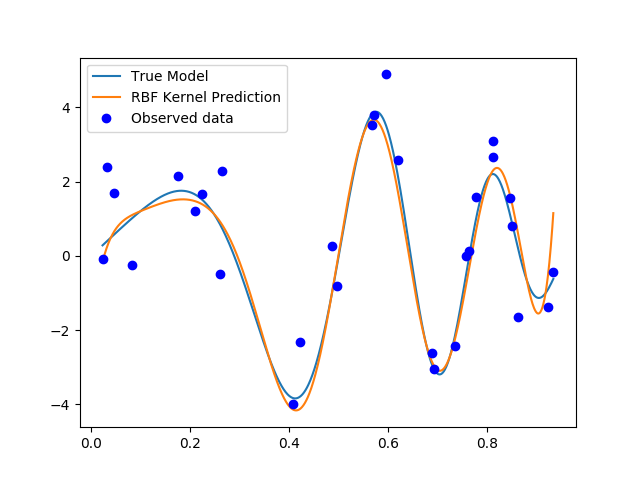
\includegraphics[width=9cm, height=6cm]{plots/A3b_2.png} 

\begin{minted}[mathescape,linenos,obeytabs=true,tabsize=2]{python}



\end{minted}

\subsection*{c.}
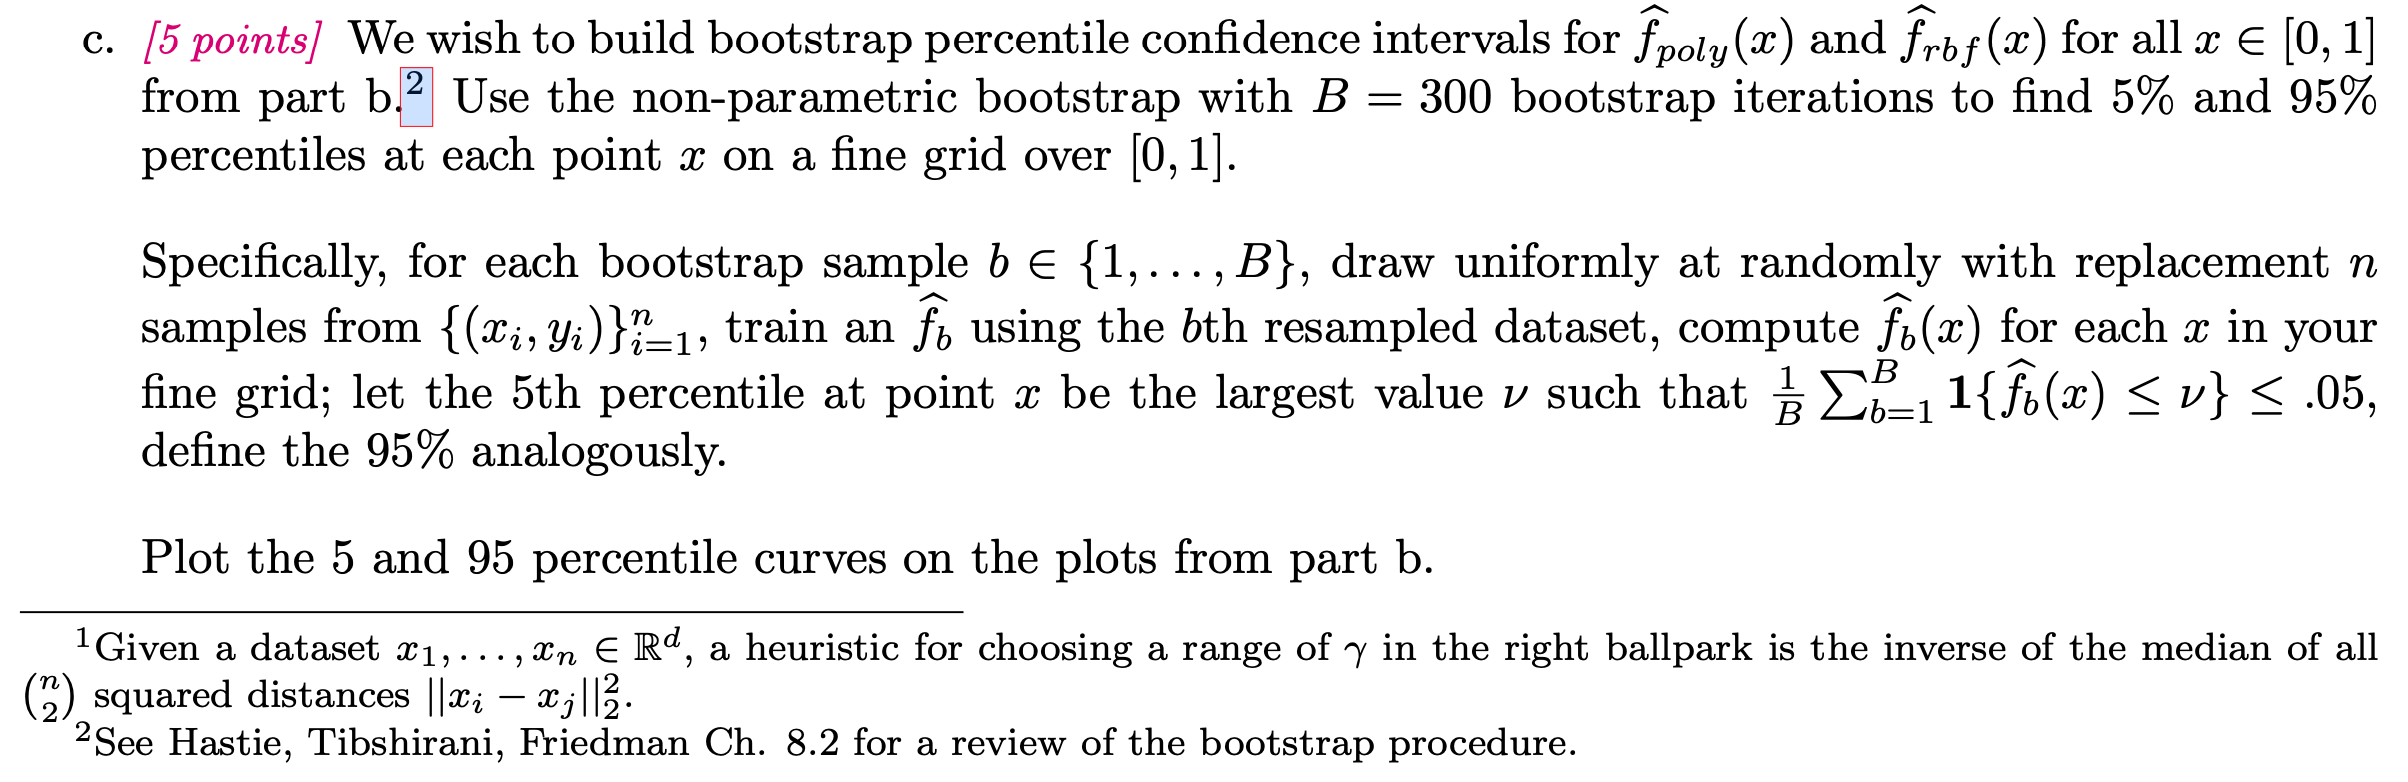
\includegraphics[width=16cm]{img/A3c.png}
\fcolorbox{red}{white}{ Solution:}

In order to train a kernel model for each re-sampled bootstrap sample, we need to compute a new alpha and K each time, according to:
\[ \hat{f} (x) = \sum_{i=1}^{n} \hat{\alpha}_i k(x_i, x) \] 

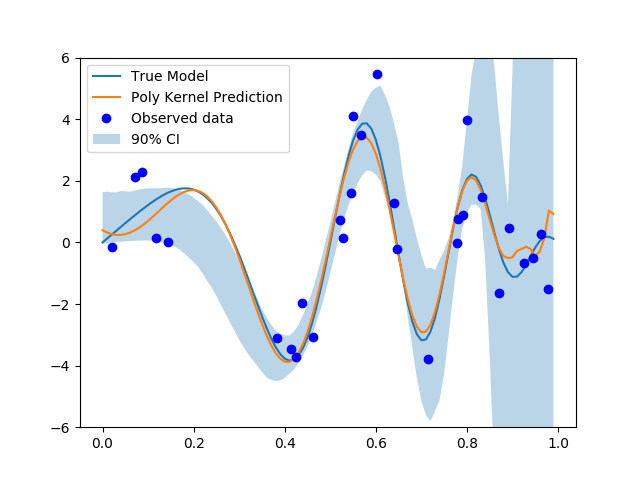
\includegraphics[width=9cm, height=6cm]{plots/A3c_1.png}
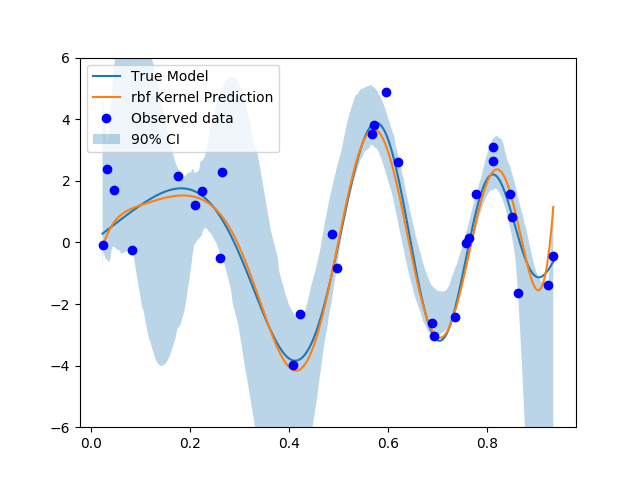
\includegraphics[width=9cm, height=6cm]{plots/A3c_2.png}


\textbf{Code for question a,b,c, } 
\begin{minted}[mathescape,linenos,obeytabs=true,tabsize=2]{python}

# b1 can also be used as part a's code
# A3.b1
import numpy as np
import matplotlib.pyplot as plt

n = 30
# np.random.seed(1)
x = np.random.uniform(0,1,n)
x_mean = np.mean(x)
x_sd = np.std(x)
# x = (x-x_mean)  # x after standardization

y = 4*np.sin(np.pi*x)*np.cos(6*np.pi*(x**2)) + np.random.standard_normal(n)
# y = (y - x_mean) / x_sd
def k_poly(x, z, d):
	a = x @ z.T
	k = (1 + x @ z.T)**d
	return k

error_validation_list = []
lamb = 500
lamb_list = []
d_list = []
for lamb in list(500 * (1/2)**(np.arange(0,20))):
	for d in list(range(0, 51)):
		error_validation = 0
		print("Lam: ", lamb, ", d: ", d)
		for i in range(n):
			x_train = np.append(x[0:i], x[i+1:n])
			y_train = np.append(y[0:i], y[i+1:n])
			x_validation = x[i]
			y_validation = y[i]
			K = k_poly(x_train[:, np.newaxis], x_train[:, np.newaxis], d)
			alpha = np.linalg.pinv(K + lamb) @ y_train
			# in predicted y formula
			k_xi_x = (1 + x_validation * x_train[np.newaxis, :]) ** d   # use this when polynomial kernel
			# k_xi_x = np.exp(-gamma*np.linalg.norm(x_validation - x_train[np.newaxis, :], 2))
			y_predicted = alpha @ k_xi_x.T
			error_validation += (y_predicted - y_validation).T @ (y_predicted- y_validation)
			# error_validation = error_validation[0][0]
		error_validation /= n
		print("error_validation: ", error_validation)
		error_validation_list.append(error_validation)
		lamb_list.append(lamb)
		d_list.append(d)

min_error = min(error_validation_list)
index_boostrap_sample_min_error = error_validation_list.index(min(error_validation_list))
lamb_best_poly = lamb_list[index_boostrap_sample_min_error]
d_best = d_list[index_boostrap_sample_min_error]
print("Best lamb: ", lamb_best_poly, ", Best d: ", d_best)

# lamb_best_poly = 0.48828125
d_best = 30
# plots the comparaison
# np.random.seed(1)
x_fine = np.array(list(np.arange(min(x),max(x), 0.01))  )
n = len(x_fine)
y_fine_true = 4*np.sin(np.pi*x_fine)*np.cos(6*np.pi*(x_fine**2))
y_fine_grid = y_fine_true + np.random.standard_normal(n)
f_poly_predicted = []
for xi in x_fine:
	K = k_poly(x_fine[:, np.newaxis], x_fine[:, np.newaxis], d_best)
	alpha = np.linalg.pinv(K + lamb_best_poly) @ y_fine_grid
	k_xi_x = (1 + xi * x_fine[np.newaxis, :]) ** d_best  # use this when polynomial kernel
	y_predicted = alpha @ k_xi_x.T
	f_poly_predicted.append(y_predicted)

plt.plot(x_fine, y_fine_true, label='True')
plt.plot(x_fine, f_poly_predicted, label='Poly Kernel')
plt.plot(x, y,'bo', label='Observed')
plt.xlabel("X")
plt.ylabel("Y")
plt.legend()
plt.savefig("/Users/yinruideng/Desktop/senior_spring/cse546/hw/hw3/latex/plots/A3b_1_test.png")
plt.show()


# A3.c1
B = 300
n = 30
n_fine = len(x_fine)
# np.random.seed(0)
boostrap_predicted_poly_matrix = []

for j in range(B):
	index_boostrap_sample = np.random.choice(n,n)
	x_training = x[index_boostrap_sample]
	y_training = y[index_boostrap_sample]
	K = k_poly(x_training[:,np.newaxis],x_training[:,np.newaxis], d_best)
	alpha = np.linalg.solve((K + lamb_best_poly*np.eye(n, n)), y_training)
	y_predicted_boostrap_ploy = []
	for xi in x_fine:
		y_predicted_boostrap_ploy.append(np.sum((1+xi*x_training[np.newaxis,:]) ** d_best @ alpha))
	boostrap_predicted_poly_matrix.append(y_predicted_boostrap_ploy)
boostrap_predicted_poly_matrix = np.array(boostrap_predicted_poly_matrix)

percent_5_list_poly = []
percent_95_list_poly = []
for i in range(n_fine):
	sorted_xi_from_300_B_sample = np.sort(boostrap_predicted_poly_matrix[:, i])
	x_percentile_5 = sorted_xi_from_300_B_sample[int(B * 0.05)]
	x_percentile_95 = sorted_xi_from_300_B_sample[int(B * 0.95)]
	percent_5_list_poly.append(x_percentile_5)
	percent_95_list_poly.append(x_percentile_95)

plt.plot(x_fine, y_fine_true, label = 'True Model')
plt.plot(x_fine, f_poly_predicted, label = 'Poly Kernel Prediction')
plt.plot(x, y,'bo', label ='Observed data')
plt.fill_between(x_fine, percent_5_list_poly, percent_95_list_poly, alpha=0.3, label="90% CI")
plt.ylim(-6, 6)
plt.legend()
plt.savefig("/Users/yinruideng/Desktop/senior_spring/cse546/hw/hw3/latex/plots/A3c_1_test.png")
plt.show()


#######################################################################################################################
# A3.b2

def k_rbf(x, z, gamma):
	return np.exp(-gamma*(x-z)*(x-z))

n = 30
# np.random.seed(0)
# x = np.random.rand(n)
x = np.random.uniform(0,1,n)
y_true = 4*np.sin(np.pi*x)*np.cos(6*np.pi*(x**2))
y = y_true + np.random.randn(n)
error_validation_list = []
lamb_list = []
gamma_list = []
d_list =[]

lamb = 1
for lamb in list(500 * (1/2)**(np.arange(0,30))):
	for gamma in list(50 * (1/1.1)**(np.arange(0,30))):
		print("Lam: ", lamb, ", gamma: ", gamma)
		error_validation = 0
		for i in range(n):
			x_train = np.append(x[0:i], x[i+1:n])
			y_train = np.append(y[0:i], y[i+1:n])
			x_validation = x[i]
			y_validation = y[i]
			K = k_rbf(x_train[:,np.newaxis],x_train[np.newaxis,:], gamma)
			alpha = np.linalg.pinv(K + lamb) @ y_train
			k_xi_x = np.exp(-gamma*(x_validation-x_train[np.newaxis,:])**2)
			error_validation += (k_xi_x@alpha - y_validation).T@(k_xi_x@alpha - y_validation)
		error_validation_list.append(error_validation)
		print("error_validation: ", error_validation)
		lamb_list.append(lamb)
		gamma_list.append(gamma)

min_error = min(error_validation_list)
index_boostrap_sample_min_error = error_validation_list.index(min_error)
lamb_best_rbf = lamb_list[index_boostrap_sample_min_error]
gamma_best = gamma_list[index_boostrap_sample_min_error]
print('Best gamma for RBF kernel is : ', gamma_best)
print('Best Lambda for RBF kernel is :', lamb_best_rbf)


gamma_best= 10.175399541327897
lamb_best_rbf= 9.313225746154785e-07
# np.random.seed(10)

x_fine = np.arange(min(x),max(x),0.001)
n = len(x_fine)
y_fine_true = 4*np.sin(np.pi*x_fine)*np.cos(6*np.pi*(x_fine**2))
y_fine_grid = y_fine_true + np.random.standard_normal(n)

f_rbf_predicted = []
K_rbf = k_rbf(x_fine[:,np.newaxis],x_fine[np.newaxis,:], gamma_best)
alpha = np.linalg.solve((K_rbf + lamb_best_rbf*np.eye(n, n)), y_fine_grid)
for xi in x_fine:
	f_rbf_predicted.append(np.sum(alpha * np.exp(-gamma_best*(xi-x_fine)**2)))

plt.plot(x_fine, y_fine_true, label = 'True Model')
plt.plot(x_fine, f_rbf_predicted, label = 'RBF Kernel Prediction')
plt.plot(x, y,'bo', label ='Observed data')
plt.legend()
plt.savefig("/Users/yinruideng/Desktop/senior_spring/cse546/hw/hw3/latex/plots/A3b_2.png")
plt.show()

# A3.c2
B = 300
n=30
n_fine = len(x_fine)
# np.random.seed(0)
boostrap_predicted_rbf_matrix = []
# user x, y from previous
for j in range(B):
	index_boostrap_sample = np.random.choice(n,n)
	x_training = x[index_boostrap_sample]
	y_training = y[index_boostrap_sample]
	K_rbf = k_rbf(x_training[:, np.newaxis], x_training[np.newaxis, :], gamma_best)
	alpha = np.linalg.solve((K_rbf + lamb_best_rbf * np.eye(n, n)), y_training)
	
	y_predicted_boostrap_rbf = []
	for xi in x_fine:
		y_predicted_boostrap_rbf.append(np.sum(alpha * np.exp(-gamma_best*(xi-x_training)**2)))
boostrap_predicted_rbf_matrix.append(y_predicted_boostrap_rbf)
boostrap_predicted_rbf_matrix = np.array(boostrap_predicted_rbf_matrix)

percent_5_list_rbf = []
percent_95_list_rbf = []
for i in range(n_fine):
	sorted_xi_from_300_B_sample = np.sort(boostrap_predicted_rbf_matrix[:, i])
	x_percentile_5 = sorted_xi_from_300_B_sample[int(B * 0.05)]
	x_percentile_95 = sorted_xi_from_300_B_sample[int(B * 0.95)]
	percent_5_list_rbf.append(x_percentile_5)
	percent_95_list_rbf.append(x_percentile_95)


plt.plot(x_fine, y_fine_true, label = 'True Model')
plt.plot(x_fine, f_rbf_predicted, label = 'rbf Kernel Prediction')
plt.plot(x, y,'bo', label ='Observed data')
plt.fill_between(x_fine, percent_5_list_rbf, percent_95_list_rbf, alpha=0.3, label="90% CI")
plt.ylim(-6, 6)
plt.legend()
plt.savefig("/Users/yinruideng/Desktop/senior_spring/cse546/hw/hw3/latex/plots/A3c_2_test.png")
plt.show()
#######################################################################################################################




\end{minted}


\subsection*{d.}
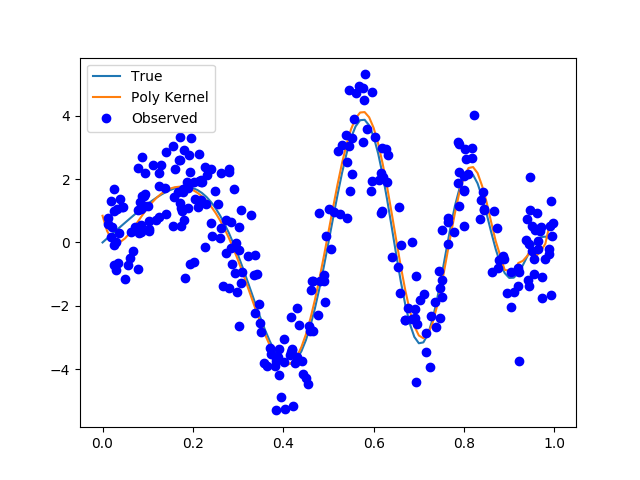
\includegraphics[width=9cm, height=6cm]{plots/A3d_1.png}
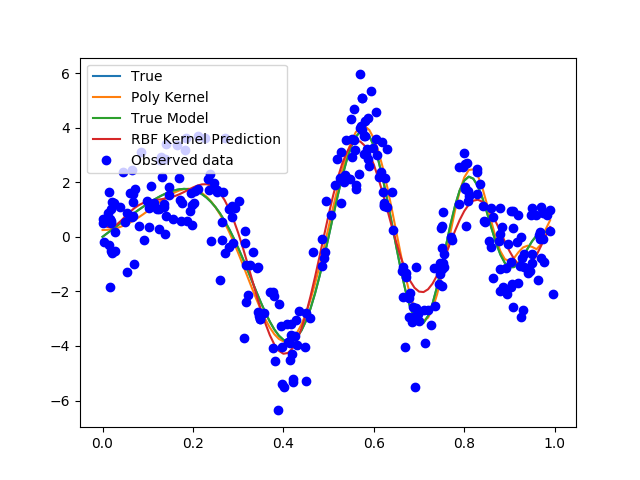
\includegraphics[width=9cm, height=6cm]{plots/A3d_2.png} \newline

Best lamb:  0.003814697265625 , Best d:  33 \\

Best gamma for RBF kernel is :  8.992939495460687 \\
Best Lambda for RBF kernel is : 1.862645149230957e-06 \\
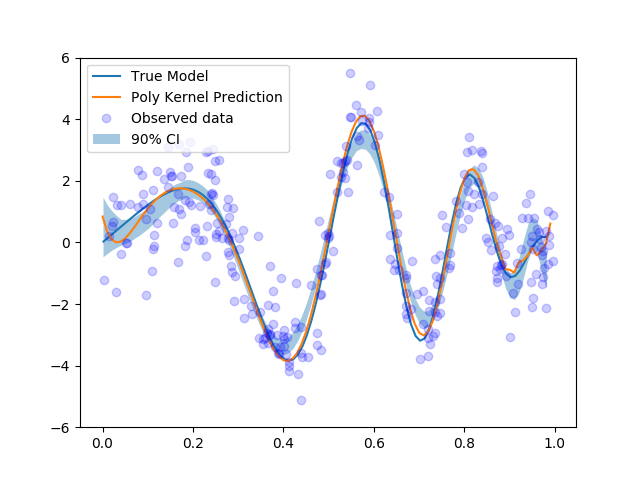
\includegraphics[width=9cm, height=6cm]{plots/A3e_1.png}
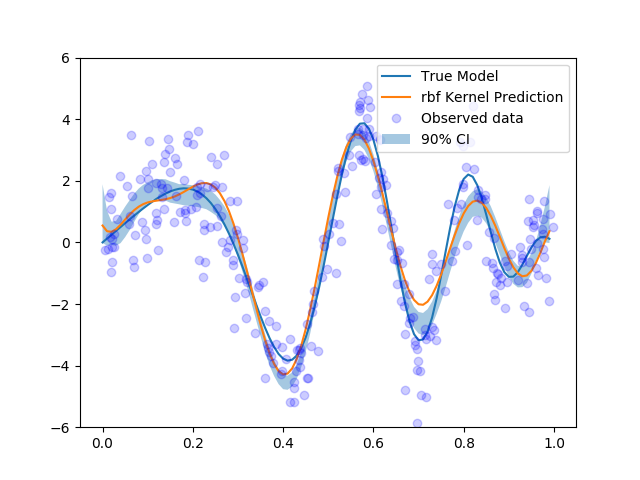
\includegraphics[width=9cm, height=6cm]{plots/A3e_2.png}

\subsection*{e.}

5\%:  -0.14401336443720553 \\
95\%:  -0.0253960255137911 \\
In my case, 0 is not included in the confidence interval. And since the 5\% and 95\% are negative, so it is suggesting that with 90\% confidence that RBF kernel is better than Polynomial kernel regression.

\textbf{Code for question d,e, } 
\begin{minted}[mathescape,linenos,obeytabs=true,tabsize=2]{python}

# A3.d - 1 #################################################################################
import numpy as np
import matplotlib.pyplot as plt

n = 300
# np.random.seed(1)

x = np.random.uniform(0,1,n)
y = 4*np.sin(np.pi*x)*np.cos(6*np.pi*(x**2)) + np.random.standard_normal(n)

def k_poly(x, z, d):
	a = x @ z.T
	k = (1 + x @ z.T)**d
	return k

error_validation_list = []
lamb = 500
cv_size = int(n/10)
lamb_list = []
d_list = []
for lamb in list(500 * (1/2)**(np.arange(0, 20))):
	for d in list(range(0, 51)):
		error_validation = 0
		print("Lam: ", lamb, ", d: ", d)
		for i in range(0, n, cv_size):
			x_train = np.append(x[0:i], x[i+cv_size:n])
			y_train = np.append(y[0:i], y[i+cv_size:n])
			x_validation = x[i:i+cv_size]
			y_validation = y[i:i+cv_size]
			K = k_poly(x_train[:, np.newaxis], x_train[:, np.newaxis], d)
			alpha = np.linalg.pinv(K + lamb) @ y_train
			# in predicted y formula
			k_xi_x = (1 + np.multiply(x_validation, np.repeat(x_train[np.newaxis, :], 
							cv_size).reshape(270,cv_size)))**d
			# y_predicted = alpha @ k_xi_x.T
			y_predicted = alpha[np.newaxis, :] @ k_xi_x
			error_validation += np.sum((y_predicted - y_validation).T @ (y_predicted- y_validation))
			# error_validation = error_validation[0][0]
			error_validation /= n
		print("error_validation: ", error_validation)
		error_validation_list.append(error_validation)
		lamb_list.append(lamb)
		d_list.append(d)

# min_error = min(error_validation_list)
index_boostrap_sample_min_error = error_validation_list.index(min(error_validation_list))
lamb_best_poly = lamb_list[index_boostrap_sample_min_error]
d_best = d_list[index_boostrap_sample_min_error]
print("Best lamb: ", lamb_best_poly, ", Best d: ", d_best)

# Best lamb:  0.003814697265625 , Best d:  40

# plots the comparaison
np.random.seed(1)
n = 100
x_fine = np.array(list(range(0, 100, 1))) / 100
y_fine_true = 4*np.sin(np.pi*x_fine)*np.cos(6*np.pi*(x_fine**2))
y_fine_grid = y_fine_true + np.random.standard_normal(n)
f_poly_predicted = []
for xi in x_fine:
	K = k_poly(x_fine[:, np.newaxis], x_fine[:, np.newaxis], d_best)
	alpha = np.linalg.pinv(K + lamb_best_poly) @ y_fine_grid
	k_xi_x = (1 + xi * x_fine[np.newaxis, :]) ** d_best  # use this when polynomial kernel
	y_predicted = alpha @ k_xi_x.T
	
	f_poly_predicted.append(y_predicted)

plt.plot(x_fine, y_fine_true, label='True')
plt.plot(x_fine, f_poly_predicted, label='Poly Kernel')
plt.plot(x, y,'bo', label='Observed')
plt.legend()
plt.savefig("/Users/yinruideng/Desktop/senior_spring/cse546/hw/hw3/latex/plots/A3d_1_test.png")
plt.show()

# -------------------------------- #

B = 300
n=300
m = 1000
x_fine = np.arange(min(x),max(x),0.01)
n_fine = len(x_fine)
# np.random.seed(10)
boostrap_predicted_poly_matrix = []
x = np.random.uniform(0,1,n)
y_true_sample = 4*np.sin(np.pi*x)*np.cos(6*np.pi*(x**2))
y_observed = y_true_sample + np.random.randn(n)

for j in range(B):
	index_boostrap_sample = np.random.choice(n,n)
	x_training = x[index_boostrap_sample]
	y_training = y_observed[index_boostrap_sample]
	K = k_poly(x_training[:,np.newaxis],x_training[:,np.newaxis], d_best)
	alpha = np.linalg.solve((K + lamb_best_poly*np.eye(n, n)), y_training)
	y_predicted_boostrap_ploy = []
	# for xi in np.array(list(range(0, 100, 1))) / 100:
	# test
	K = k_poly(x_training[:,np.newaxis],x_training[:,np.newaxis], d_best)
	alpha = np.linalg.solve((K + lamb_best_poly*np.eye(n, n)), y_training)
	
	for xi in x_fine:
		y_predicted_boostrap_ploy.append(np.sum((1+xi*x_training[np.newaxis,:]) ** d_best @ alpha))
	boostrap_predicted_poly_matrix.append(y_predicted_boostrap_ploy)
boostrap_predicted_poly_matrix = np.array(boostrap_predicted_poly_matrix)

percent_5_list_poly = []
percent_95_list_poly = []
for i in range(n_fine):
	sorted_xi_from_300_B_sample = np.sort(boostrap_predicted_poly_matrix[:, i])
	x_percentile_5 = sorted_xi_from_300_B_sample[int(B * 0.05)]
	x_percentile_95 = sorted_xi_from_300_B_sample[int(B * 0.95)]
	percent_5_list_poly.append(x_percentile_5)
	percent_95_list_poly.append(x_percentile_95)

# x_fine = np.array(list(range(0, 100, 1))) / 100
y_fine_true = 4*np.sin(np.pi*x_fine)*np.cos(6*np.pi*(x_fine**2))
plt.plot(x_fine, y_fine_true, label = 'True Model')
plt.plot(np.array(list(range(0, 100, 1))) / 100, f_poly_predicted, label = 'Poly Kernel Prediction')
plt.fill_between(x_fine, percent_5_list_poly, percent_95_list_poly, alpha=0.4, label="90% CI")
plt.plot(x, y_observed,'bo', alpha=0.2, label ='Observed data')
plt.ylim(-6, 6)
plt.legend()
plt.savefig("/Users/yinruideng/Desktop/senior_spring/cse546/hw/hw3/latex/plots/A3e_1_test.png")
plt.show()



###################################################################################################################

# A3.d - 2

def k_rbf(x, z, gamma):
	return np.exp(-gamma*(x-z)*(x-z))

n = 300
np.random.seed(1)
cv_size = int(n/10)
x = np.random.uniform(0,1,n)
y_true = 4*np.sin(np.pi*x)*np.cos(6*np.pi*(x**2))
y = y_true + np.random.randn(n)
error_validation_list = []
lamb_list = []
gamma_list = []
d_list =[]

lamb = 1
for lamb in list(500 * (1/2)**(np.arange(0,30))):
	for gamma in list(50 * (1/1.1)**(np.arange(0,30))):
		print("Lam: ", lamb, ", gamma: ", gamma)
		error_validation = 0
		for i in range(0, n, cv_size):
			x_train = np.append(x[0:i], x[i+cv_size:n])
			y_train = np.append(y[0:i], y[i+cv_size:n])
			x_validation = x[i:i+cv_size]
			y_validation = y[i:i+cv_size]
			K = k_rbf(x_train[:,np.newaxis],x_train[np.newaxis,:], gamma)
			alpha = np.linalg.pinv(K + lamb) @ y_train
			k_xi_x = np.exp(-gamma*(x_validation - np.repeat(x_train[np.newaxis,:], 
							cv_size).reshape((n-cv_size, cv_size)))**2)
			y_predicted = alpha[np.newaxis, :] @ k_xi_x
			error_validation += np.sum((y_predicted - y_validation).T @ (y_predicted- y_validation))
		error_validation /= n
		error_validation_list.append(error_validation)
		print("error_validation: ", error_validation)
		lamb_list.append(lamb)
		gamma_list.append(gamma)

min_error = min(error_validation_list)
index_boostrap_sample_min_error = error_validation_list.index(min_error)
lamb_best_rbf = lamb_list[index_boostrap_sample_min_error]
gamma_best = gamma_list[index_boostrap_sample_min_error]
print('Best gamma for RBF kernel is : ', gamma_best)
print('Best Lambda for RBF kernel is :', lamb_best_rbf)

# Best gamma for RBF kernel is :  8.992939495460687
# Best Lambda for RBF kernel is : 1.862645149230957e-06
# plots the comparaison
n = 100
np.random.seed(10)

x_fine = np.array(list(range(0, 100, 1))) / 100
y_fine_true = 4*np.sin(np.pi*x_fine)*np.cos(6*np.pi*(x_fine**2))
y_fine_grid = y_fine_true + np.random.standard_normal(n)

f_rbf_predicted = []
K_rbf = k_rbf(x_fine[:,np.newaxis],x_fine[np.newaxis,:], gamma_best)
alpha = np.linalg.solve((K_rbf + lamb_best_rbf*np.eye(n, n)), y_fine_grid)
for xi in x_fine:
	f_rbf_predicted.append(np.sum(alpha * np.exp(-gamma_best*(xi-x_fine)**2)))

plt.plot(x_fine, y_fine_true, label = 'True Model')
plt.plot(x_fine, f_rbf_predicted, label = 'RBF Kernel Prediction')
plt.plot(x, y,'bo', label ='Observed data')
plt.legend()
plt.savefig("/Users/yinruideng/Desktop/senior_spring/cse546/hw/hw3/latex/plots/A3d_2_test.png")
plt.show()


# A3.e2
B = 300
n=300
# m=1000
# n_fine = 100
np.random.seed(0)
boostrap_predicted_rbf_matrix = []
# x = np.array(list(range(0, 100, 1))) / 100
x = np.random.uniform(0,1,n)
y_true_sample = 4*np.sin(np.pi*x)*np.cos(6*np.pi*(x**2))
y_observed = y_true_sample + np.random.randn(n)

for j in range(B):
	index_boostrap_sample = np.random.choice(n,n)
	x_training = x[index_boostrap_sample]
	y_training = y_observed[index_boostrap_sample]
	K_rbf = k_rbf(x_training[:, np.newaxis], x_training[np.newaxis, :], gamma_best)
	alpha = np.linalg.solve((K_rbf + lamb_best_rbf * np.eye(n, n)), y_training)
	
	y_predicted_boostrap_rbf = []
	for xi in x_fine:
		# k_xi_x = np.exp(-gamma * (xi - x_training[np.newaxis, :]) ** 2)
		# predicted = k_xi_x@alpha
		y_predicted_boostrap_rbf.append(np.sum(alpha * np.exp(-gamma_best*(xi-x_training)**2)))
	boostrap_predicted_rbf_matrix.append(y_predicted_boostrap_rbf)
boostrap_predicted_rbf_matrix = np.array(boostrap_predicted_rbf_matrix)

percent_5_list_rbf = []
percent_95_list_rbf = []
for i in range(len(x_fine)):
	sorted_xi_from_300_B_sample = np.sort(boostrap_predicted_rbf_matrix[:, i])
	x_percentile_5 = sorted_xi_from_300_B_sample[int(B * 0.05)]
	x_percentile_95 = sorted_xi_from_300_B_sample[int(B * 0.95)]
	percent_5_list_rbf.append(x_percentile_5)
	percent_95_list_rbf.append(x_percentile_95)

x_fine = np.array(list(range(0, 100, 1))) / 100
y_fine_true = 4*np.sin(np.pi*x_fine)*np.cos(6*np.pi*(x_fine**2))
plt.plot(x_fine, y_fine_true, label = 'True Model')
plt.plot(x_fine, f_rbf_predicted, label = 'rbf Kernel Prediction')
plt.fill_between(x_fine, percent_5_list_rbf, percent_95_list_rbf, alpha=0.4, label="90% CI")
plt.plot(x, y_observed,'bo', alpha=0.2, label ='Observed data')
plt.ylim(-6, 6)
plt.legend()
plt.savefig("/Users/yinruideng/Desktop/senior_spring/cse546/hw/hw3/latex/plots/A3e_2_test.png")
plt.show()







########################################## A3 e ##########################################
#
#                                          A3 e
#
########################################## A3 e ##########################################
d_best=33

B = 300
n=300
m=1000
np.random.seed(4)
x = np.random.uniform(0,1,m+n)
y_true_sample = 4*np.sin(np.pi*x)*np.cos(6*np.pi*(x**2))
y_observed = y_true_sample + np.random.randn(m+n)
error_difference_list = np.zeros(B)

for j in range(B):
	print("B: ", j)
	index_boostrap_sample = np.random.choice(m+n,m)
	x_training = x[index_boostrap_sample]
	y_training = y_observed[index_boostrap_sample]
	# comput poly kernel
	K = k_poly(x_training[:, np.newaxis], x_training[:, np.newaxis], d_best)
	alpha = np.linalg.pinv(K + lamb_best_poly) @ y_training
	# compute rbf kernel
	K_rbf = k_rbf(x_training[:, np.newaxis], x_training[np.newaxis, :], gamma_best)
	alpha_rbf = np.linalg.solve((K_rbf + lamb_best_rbf * np.eye(m, m)), y_training)
	
	error_difference = 0
	for i in range(len(x_training)):
		# poly predicted
		k_xi_x = (1 + x_training[i] * x_training[np.newaxis, :]) ** d_best  # use this when polynomial kernel
		y_predicted = alpha @ k_xi_x.T
		# rbf predicted
		y_predicted_rbf = np.sum(alpha_rbf * np.exp(-gamma_best*(x_training[i]-x_training)**2))
		# error difference
		error_difference += (y_training[i] - y_predicted)**2 - (y_training[i] - y_predicted_rbf)**2
	error_difference /= len(x_training)
	# error_difference_list.append(error_difference)
	print("error_difference: ", error_difference)
	error_difference_list[j] = error_difference
	error_difference_list = np.sort(error_difference_list)

print("5%: ", error_difference_list[int(B * 0.05)])
print("95%: ", error_difference_list[int(B * 0.95)])


\end{minted}





\section*{A.4}


\subsection*{a.}
\begin{minted}[mathescape,linenos,obeytabs=true,tabsize=2]{python}
import numpy as np
import matplotlib.pyplot as plt
from mnist import MNIST
import random

def load_data(size=1):
	print("Loading Date!")
	mndata = MNIST('python-mnist/data/')
	X_train, labels_train = map(np.array, mndata.load_training())
	X_test, labels_test = map(np.array, mndata.load_testing())
	X_train = X_train / 255.0
	X_test = X_test / 255.0
	
	if (size != 1):
		return X_train[:int(len(X_train)*size)], \
		labels_train[:int(len(labels_train)*size)], \
		X_test[:int(len(X_test)*size)], \
		labels_test[:int(len(labels_test)*size)]
	else:
		return X_train, labels_train, X_test, labels_test
X_train, y_train, X_test, y_test = load_data(size=0.1)
print("Load Data Compelete!")

def compute_cluster(X_train, centers, k):
	objective_value = 0
	clusters = [[] for i in range(k)]
	for i in np.arange(len(X_train)):
		distance_list = []
		for center in centers:
			norm = np.linalg.norm(X_train[i] - center)
			distance_list.append(norm)
		closesed_center_index = distance_list.index(min(distance_list))
		objective_value += min(distance_list)**2
		clusters[closesed_center_index].append(X_train[i])
	return clusters, objective_value

def compute_centers(classes):
	centers = []
	for i in range(len(classes)):
		centers.append(np.mean(classes[i], axis = 0))
	return centers

objective_value_list = []

k = 10
objs = []
iteration = 0
old_centers = random.sample(list(X_train), k)
new_centers = random.sample(list(X_train), k)
while not np.array_equal(old_centers, new_centers):
	iteration += 1
	print("Iteration: ", iteration)
	print("----------  Compute Clusters -----------")
	old_centers = new_centers
	clusters, objective_value = compute_cluster(X_train, new_centers, k)
	print("objective_value: ", objective_value)
	new_centers = compute_centers(clusters)
	objective_value_list.append(objective_value)

\end{minted}

\subsection*{b.}
\begin{minted}[mathescape,linenos,obeytabs=true,tabsize=2]{python}
# plot center imgs
for i in range(k):
	plt.imshow(new_centers[i].reshape((28, 28)))
	plt.savefig("/Users/yinruideng/Desktop/senior_spring/cse546/hw/hw3/latex/plots/A4/A4b_"+
	str(i)+".png")
plt.show()
\end{minted}

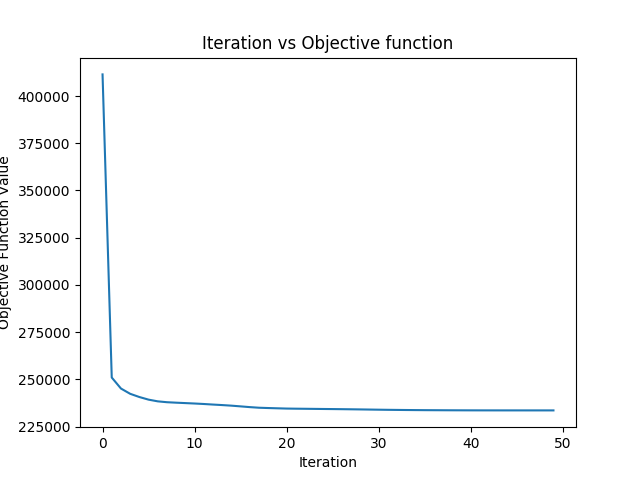
\includegraphics[width=9cm, height=6cm]{plots/A4/A4b.png} \newline
When K = 10, the centroids are:

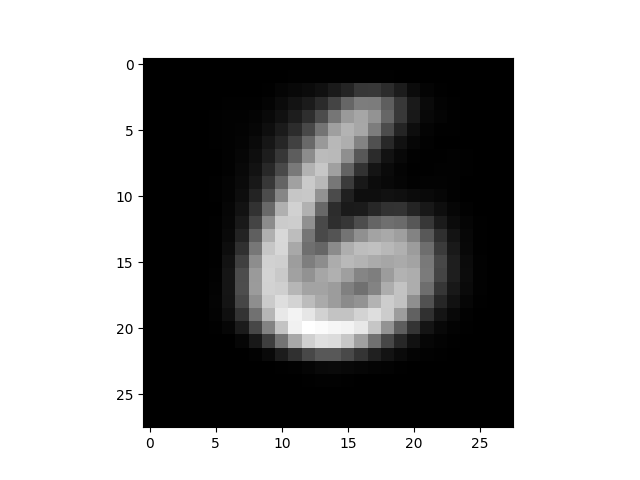
\includegraphics[width=1.8cm, height=2cm]{plots/A4/A4b_0.png}
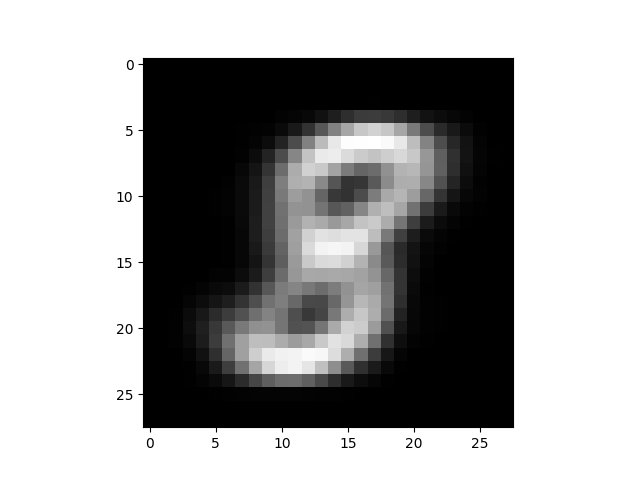
\includegraphics[width=1.8cm, height=2cm]{plots/A4/A4b_1.png}
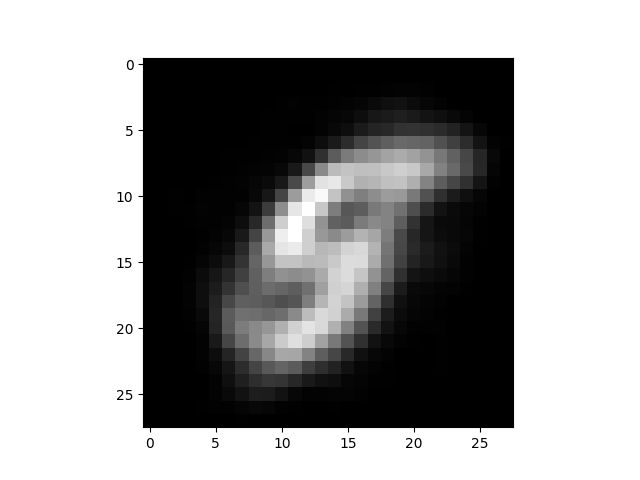
\includegraphics[width=1.8cm, height=2cm]{plots/A4/A4b_2.png}
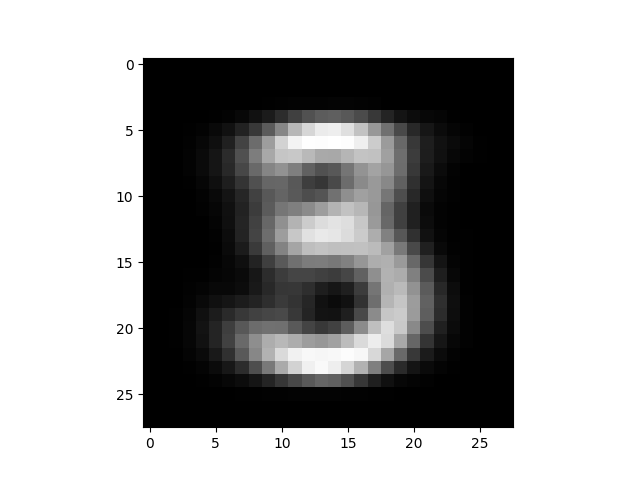
\includegraphics[width=1.8cm, height=2cm]{plots/A4/A4b_3.png}
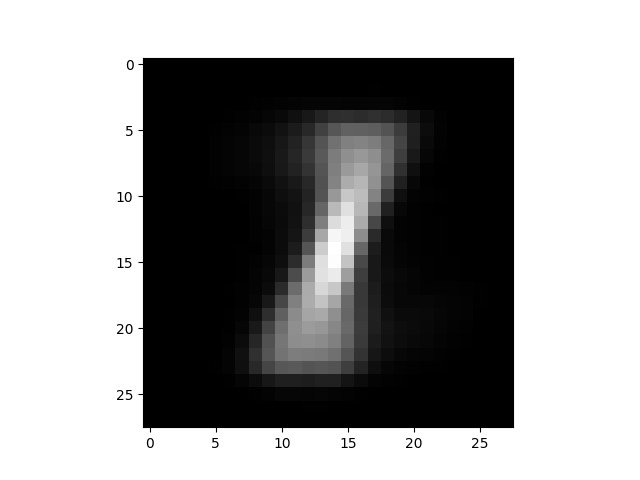
\includegraphics[width=1.8cm, height=2cm]{plots/A4/A4b_4.png}
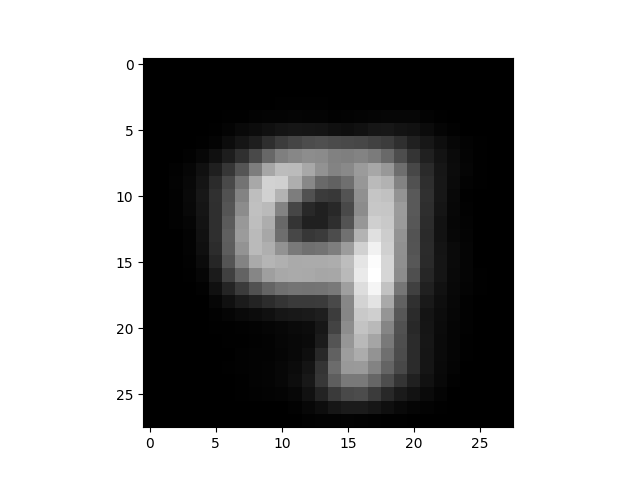
\includegraphics[width=1.8cm, height=2cm]{plots/A4/A4b_5.png}
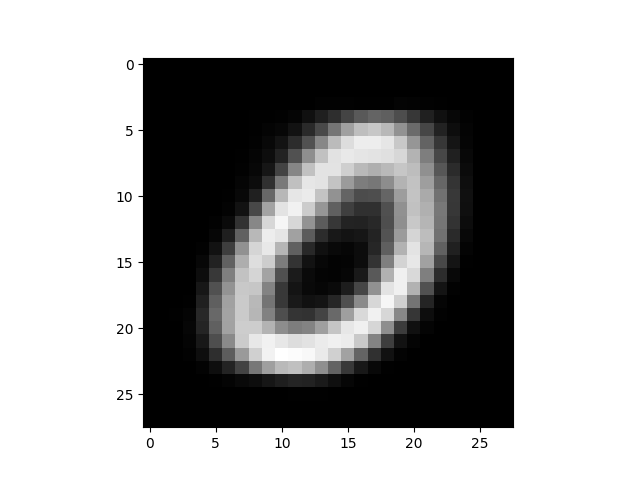
\includegraphics[width=1.8cm, height=2cm]{plots/A4/A4b_6.png}
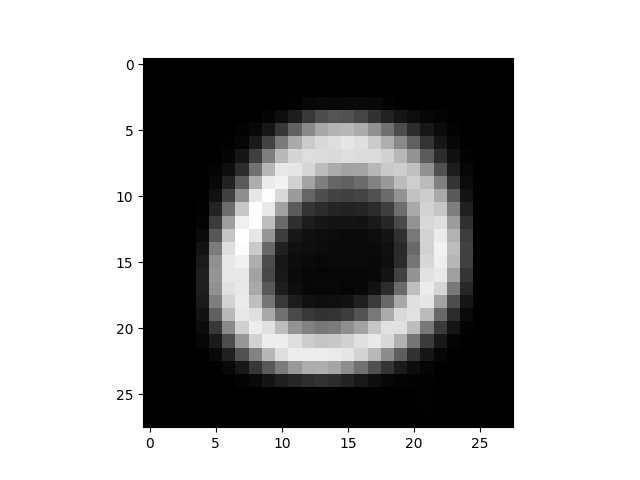
\includegraphics[width=1.8cm, height=2cm]{plots/A4/A4b_7.png}
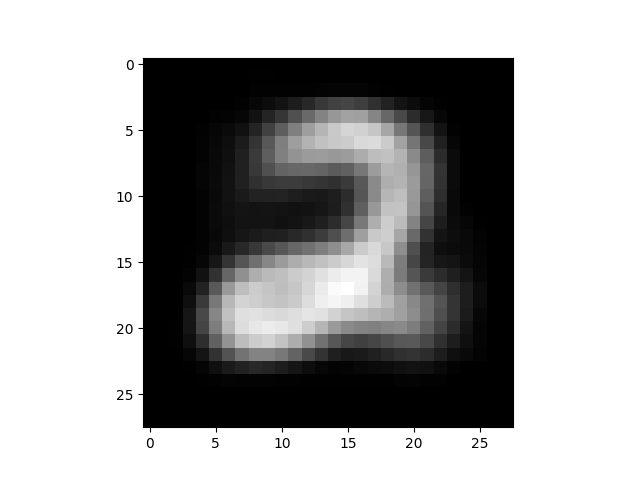
\includegraphics[width=1.8cm, height=2cm]{plots/A4/A4b_8.png}
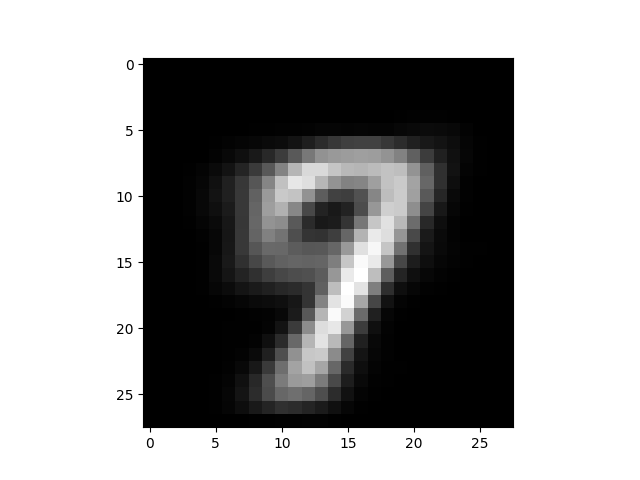
\includegraphics[width=1.8cm, height=2cm]{plots/A4/A4b_9.png}


\subsection*{c.}
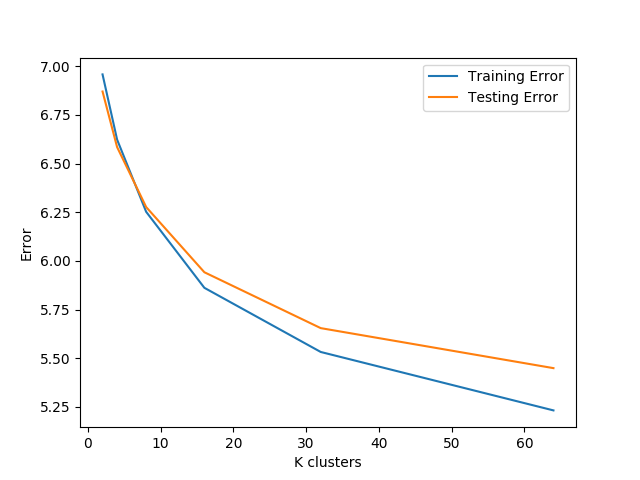
\includegraphics[width=9cm, height=6cm]{plots/A4/A4c.png} \newline

\begin{minted}[mathescape,linenos,obeytabs=true,tabsize=2]{python}
objective_value_list = []
training_error_list = []
testing_error_list = []
k_list = [2,4,8,16,32,64]

for k in k_list:
	objs = []
	iteration = 0
	old_centers = random.sample(list(X_train), k)
	new_centers = random.sample(list(X_train), k)
	while not np.array_equal(old_centers, new_centers):
		iteration += 1
		print("Iteration: ", iteration)
		print("----------  Compute Clusters -----------")
		old_centers = new_centers
		clusters, objective_value = compute_cluster(X_train, new_centers, k)
		print("objective_value: ", objective_value)
		new_centers = compute_centers(clusters)
		objective_value_list.append(objective_value)
	training_error = 0
	for x_i in X_train:
		distance_to_center = [np.linalg.norm(x_i - center) for center in new_centers]
		training_error += min(distance_to_center)
	training_error /= len(X_train)
	training_error_list.append(training_error)
		
	testing_error = 0
	for x_i in X_test:
		distance_to_center = [np.linalg.norm(x_i - center) for center in new_centers]
		testing_error += min(distance_to_center)
	testing_error /= len(X_test)
	testing_error_list.append(testing_error)

plt.plot(k_list, training_error_list, label="Training Error")
plt.plot(k_list, testing_error_list, label="Testing Error")
plt.ylabel("Error")
plt.xlabel("K clusters")
plt.legend()
plt.savefig("/Users/yinruideng/Desktop/senior_spring/cse546/hw/hw3/latex/plots/A4/A4c.png")
plt.show()
\end{minted}




\section*{B.1}

\subsection*{a.}
From the hint, we get to know that:
\[ 1- \epsilon \le e^{-\epsilon} \]
Then based on for some $f_i \in \mathcal{F}$, we have $R(f_i) > \epsilon$,
\[ 1- \epsilon \le e^{-\epsilon} \]
\[ 1 - e^{-\epsilon} \le \epsilon \] 
\[ 1 - e^{-\epsilon} \le \epsilon < R(f_i) \]
\[ 1 - e^{-\epsilon} \le R(f_i) \]
\[ e^{-\epsilon} -1 \ge - R(f_i) \]
\[ e^{-\epsilon} \ge 1 - R(f_i) \]
\[ e^{-\epsilon} \ge 1 - E \bigg[ \mathds{1} \{ f(x_1) \neq y_i \} \bigg] \]
\[ e^{-\epsilon} \ge 1 - P \bigg[ \hat{R}_n (f_i) \neq 0 \bigg] \]
\[ e^{-\epsilon} \ge P \bigg[ \hat{R}_n (f_i) = 0 \bigg] \]
\[ (e^{-\epsilon})^n \ge (P \bigg[ \hat{R}_n (f_i) = 0 \bigg] )^n\]
\[ e^{-n\epsilon} \ge P \bigg[ \hat{R}_n (f) = 0 \bigg] \]


\subsection*{b.}
Suppose there are k $f_i$ satisfy the requirement and Let event:
\[ A_i = \{ R(f_i) > \epsilon \text{ and } \hat{R}_n(f) = 0 \} \] 
And from previous question we know that:
\[ Pr\big( \hat{R}_n(f) = 0 \big) \le e^{-n\epsilon} \]
So this works as well,
\[ Pr\big( \hat{R}_n(f) = 0 \big) * Pr\big( R(f_i) > \epsilon \big) \le e^{-n\epsilon} \]
\[ Pr(A_i)  \le e^{-n\epsilon} \]
\[ Pr(A_1 \cup A_2 \cup A_3 \dots \cup A_n)  \le \sum_{i=1}^{i=k} A_i \]
\[ Pr(A_1 \cup A_2 \cup A_3 \dots \cup A_n)  \le \sum e^{-n\epsilon} \]
\[ Pr(A_1 \cup A_2 \cup A_3 \dots \cup A_n)  \le k e^{-n\epsilon} \]
So,
\[ \prod Pr\big( R(f_i) > \epsilon \text{ and } \hat{R}_n(f) =0 \big) \le |\mathcal{F}| e^{-n\epsilon}\]

\[ Pr\big( \exists f \in \mathcal{F} s.t R(f) > \epsilon \text{ and } \hat{R}_n(f) =0 \big) \le |\mathcal{F}| e^{-n\epsilon}\]

\subsection*{c.}

\[ |\mathcal{F}| e^{-\epsilon n} \le \delta  \]
\[ e^{-\epsilon n} \le \frac{\delta}{|\mathcal{F}|} \]
\[ -\epsilon n \le log(\frac{\delta}{|\mathcal{F}|}) \]
\[ \epsilon n \ge log(\frac{|\mathcal{F}|}{\delta}) \]
\[ \epsilon \ge \frac{1}{n} log(\frac{|\mathcal{F}|}{\delta}) \]
So,
\[ \epsilon_{min} = \frac{1}{n} log(\frac{|\mathcal{F}|}{\delta}) \]

\subsection*{d.}
According to Chebyshev Inequality, for any random variable X and $\epsilon > 0$:
\[ P( |X - E[X]| > \epsilon ) \le \frac{V[X]}{\epsilon^2}  \]
\[ P( |X - E[X]| \le \epsilon ) > \frac{V[X]}{\epsilon^2}  \]
And here: X is $ R(\hat{f}) $, \\
From previous question we got: 
\[ \epsilon \ge \frac{1}{n} log(\frac{|\mathcal{F}|}{\delta}) \]
So,
\[ P\big( R(\hat{f}) - R(f^*) \le \epsilon \big) \ge \frac{V[R(\hat{f})]}{\epsilon^2} \]
So now, we want to prove that:
\[ \frac{V[R(\hat{f})]}{\epsilon^2} \ge 1 - \delta \]
So, here is what I will do, I will use the inequality from c:
\[ \epsilon \ge  \frac{1}{n} log(\frac{|\mathcal{F}|}{\delta})  \]
\[ (\epsilon)^2 \ge ( \frac{1}{n} log(\frac{|\mathcal{F}|}{\delta}) ) ^2 \]
\[ \frac{V[R(\hat{f})]}{\epsilon^2} \ge V[R(\hat{f})] / ( \frac{1}{n} log(\frac{|\mathcal{F}|}{\delta}) ) ^2 \]
\[  \frac{V[R(\hat{f})]}{\epsilon^2} \ge \frac{n^2 V[R(\hat{f})] }{( log(|\mathcal{F}|) - log(\delta ) )^2} \]
And the variance need to be noted, variance of distribution of the best function should be smaller than the variance of the original distribution, according to the variance of distribution of sample mean $\sigma^2_{\bar{x}} = \frac{\sigma^2_{x_i}}{n} $, and same idea applies here. However, it is not nessesarily 1/n in this case, but I will just regard it this way and the inequality will still hold because we know that $V[R(f_i)]$ is bigger than $V[ R(\hat{f}) ]$. And the reason I do this is because $V[R(\hat{f})]$ might be close to 0 and I don't want the numerator to risk to be 0, if the numerator is 0, then the proof failed. So, I will use the following:
\[ V[R(\hat{f})] \approxeq \frac{V[R(f_i)]}{n} \]
So,
\[  \frac{V}{\epsilon^2} \ge \frac{n^2 \frac{V[R(f_i)]}{n} }{( log(|\mathcal{F}|) - log(\delta ) )^2} \]
\[  \frac{V}{\epsilon^2} \ge \frac{n V[R(f_i)] }{( log(|\mathcal{F}|) - log(\delta ) )^2} \]
Here, we know that $n > |\mathcal{F}|$ since $|\mathcal{F}|$ is finite, and n is infinity technically. And here $V[R(f_i)] \neq 0$. And since n is approximately infinity, and also the left hand side of the equation is positive, so:
\[ n \frac{V[R(f_i)] }{( log(|\mathcal{F}|) - log(\delta ) )^2} \ge 1 \]
\[ n \frac{ V[R(f_i)] }{( log(|\mathcal{F}|) - log(\delta ) )^2} \ge 1 - \delta \]
So, now we have proved that:
\[ \frac{V[R(\hat{f})]}{\epsilon^2} \ge 1 - \delta \]
Then,
\[ P\big( R(\hat{f}) - R(f^*) \le \epsilon \big) \ge \frac{V[R(\hat{f})]}{\epsilon^2} \ge 1 - \delta\]
Then,
\[ P\big( R(\hat{f}) - R(f^*) \le \frac{log(|\mathcal{F}| / \delta)}{n} \big) \ge \frac{V[R(\hat{f})]}{\epsilon^2} \ge 1 - \delta \]


\section*{A.5}
\subsection*{a.}
This part used a simple nn: \newline
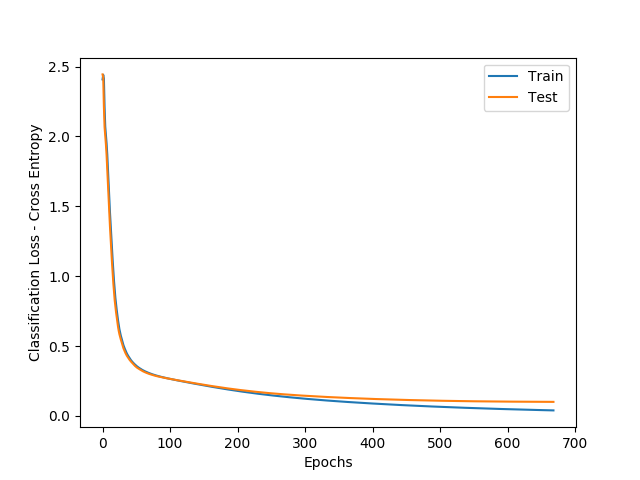
\includegraphics[width=9cm, height=6cm]{plots/A5a_2.png} 
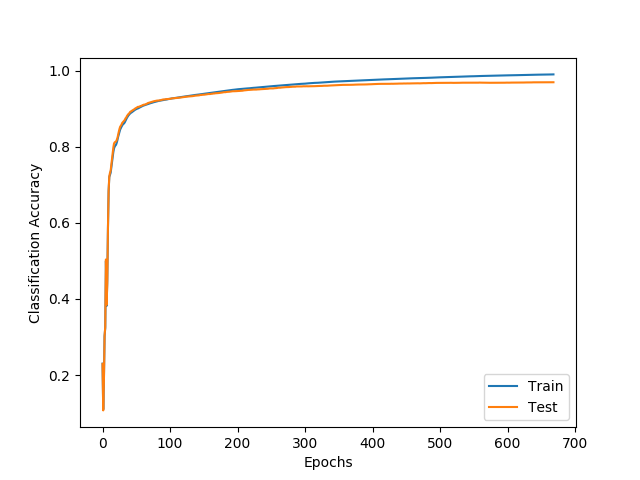
\includegraphics[width=9cm, height=6cm]{plots/A5a.png} \newline
Train Accuracy:  0.99 \newline
Test Accuracy:  0.9701\newline
Train Loss:  (0.0408)\newline
Test Loss:  (0.1029)\newline

\begin{minted}[mathescape,linenos,obeytabs=true,tabsize=2]{python}
import numpy as np
import torch
import matplotlib.pyplot as plt
from mnist import MNIST

def load_data(size=1):
	print("Loading Date!")
	mndata = MNIST('python-mnist/data/')
	X_train, labels_train = map(np.array, mndata.load_training())
	X_test, labels_test = map(np.array, mndata.load_testing())
	X_train = X_train / 255.0
	X_test = X_test / 255.0
	
	if (size != 1):
		return X_train[:int(len(X_train)*size)], \
		labels_train[:int(len(labels_train)*size)], \
		X_test[:int(len(X_test)*size)], \
		labels_test[:int(len(labels_test)*size)]
	else:
		return X_train, labels_train, X_test, labels_test

# One hot encoding
def one_hot(y_train_, m):
	n = len(y_train_)
	reformed_tensor = torch.zeros(n, m)
	for i in range(n):
		index = y_train_[i]
		reformed_tensor[i][index] = 1
	return reformed_tensor

if __name__ == "__main__":
	X_train, y_train, X_test, y_test = load_data(size=1)
	print("Load Data Compelete!")
	# convert to tensor
	dtype = torch.FloatTensor
	
	X_train_ = torch.tensor(X_train, dtype=torch.double).type(dtype)
	y_train_ = torch.tensor(y_train, dtype=torch.int64)
	
	X_test_ = torch.tensor(X_test, dtype=torch.double).type(dtype)
	y_test_ = torch.tensor(y_test, dtype=torch.int64)
	
	def ReLU(x):
		return abs(x) * (x > 0)
	
	def model(x, w0, w1, b0, b1):
		return (w1 @ ReLU(w0 @ x.T + b0) + b1).T
	
	def alpha(d):
	return 1 / np.sqrt(d)
	h = 64
	k = 10
	n_train, d_train = X_train.shape
	w0_data = (alpha(d_train) + alpha(d_train))*(torch.rand(h, d_train) -alpha(d_train)).type(dtype)
	w0 = torch.autograd.Variable(w0_data, requires_grad=True)
	b0_data = (alpha(d_train) + alpha(d_train))*(torch.rand(h, 1) -alpha(d_train)).type(dtype)
	b0 = torch.autograd.Variable(b0_data,requires_grad=True)
	w1_data = (alpha(d_train) + alpha(d_train))*(torch.rand(k, h) -alpha(d_train)).type(dtype)
	n_test, d_test = X_test.shape
	w1 = torch.autograd.Variable(w1_data,requires_grad=True)
	b1_data = (alpha(d_train) + alpha(d_train))*(torch.rand(k, 1) -alpha(d_train)).type(dtype)
	b1 = torch.autograd.Variable(b1_data, requires_grad=True)
	step_size = 0.001
	epochs = 150
	train_accuracy_list = []
	test_accuracy_list = []
	loss_train_list = []
	loss_test_list = []
	
	optim = torch.optim.Adam([w0, w1, b0, b1], lr=step_size)
	
	train_accu = 0
	test_accu = 0
	epochs_list = list(range(epochs))
	# for epoch in epochs_list:
	iter = 0
	while train_accu < 0.99:
		iter += 1
		# print("Epoch: ", epoch)
		optim.zero_grad()
		y_hat = model(X_train_, w0, w1, b0, b1)
		y_hat_index = torch.max(y_hat, dim=0).indices
		loss = torch.nn.functional.cross_entropy(y_hat, y_train_)
		loss.backward()
		optim.step()
		# Cross Entropy
		max_index_train = torch.max(model(X_train_, w0, w1, b0, b1), dim=1).indices.numpy()
		num_corrected_prediction_train = sum(max_index_train == y_train)
		train_accu = num_corrected_prediction_train / len(y_train)
		train_accuracy_list.append(train_accu)
		loss_train_list.append(loss)
		
		
		max_index_test = torch.max(model(X_test_, w0, w1, b0, b1), dim=1).indices.numpy()
		num_corrected_prediction_test = sum(max_index_test == y_test)
		test_accu = num_corrected_prediction_test / len(y_test)
		test_accuracy_list.append(test_accu)
		loss_test_list.append(torch.nn.functional.cross_entropy(model(X_test_, w0, w1, b0, b1), y_test_))
		print("##################", iter, "##################")
		print("CROSS ENTROPY: Train Accuracy: ", train_accu)
		print("CROSS ENTROPY: Test Accuracy: ", test_accu)
		
	print("CROSS ENTROPY: Train Accuracy: ", train_accuracy_list[-1])
	print("CROSS ENTROPY: Test Accuracy: ", test_accuracy_list[-1])
	print("Train Loss: ", loss_train_list[-1])
	print("Test Loss: ", loss_test_list[-1])
	
	plt.plot(range(iter), train_accuracy_list, label="Train")
	plt.plot(range(iter), test_accuracy_list, label="Test")
	plt.xlabel("Epochs")
	plt.ylabel("Classification Accuracy - Cross Entropy")
	plt.legend()
	plt.savefig("/Users/yinruideng/Desktop/senior_spring/cse546/hw/hw3/latex/plots/A5a.png")
	plt.show()
	
	w0.shape[0] * w0.shape[1] + w1.shape[0] * w1.shape[1] + len(b0) + len(b1)




\end{minted}


\subsection*{b.}
This part used a little more complex nn than last part: \newline
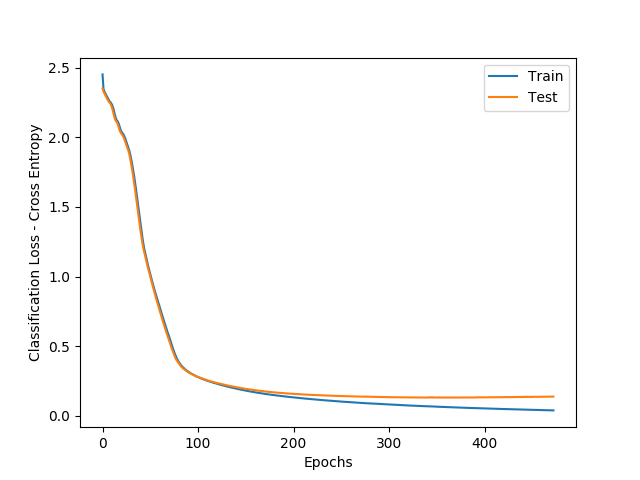
\includegraphics[width=9cm, height=6cm]{plots/A5b_2.png} 
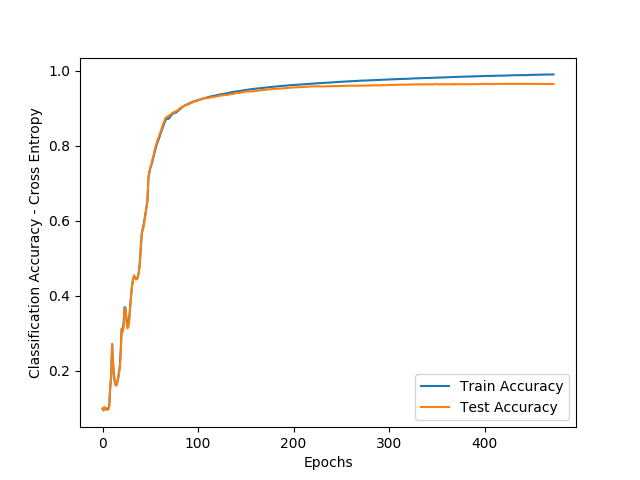
\includegraphics[width=9cm, height=6cm]{plots/A5b.png} \newline
Train Accuracy:  0.99005\newline
Test Accuracy:  0.9624\newline
Train Loss:  (0.0409)\newline
Test Loss:  (0.1531)\newline

\begin{minted}[mathescape,linenos,obeytabs=true,tabsize=2]{python}
import numpy as np
import torch
import matplotlib.pyplot as plt
from mnist import MNIST


if __name__ == "__main__":
	X_train, y_train, X_test, y_test = load_data(size=1)
	print("Load Data Compelete!")
	# convert to tensor
	dtype = torch.FloatTensor
	
	X_train_ = torch.tensor(X_train, dtype=torch.double).type(dtype)
	y_train_ = torch.tensor(y_train, dtype=torch.int64)
	
	X_test_ = torch.tensor(X_test, dtype=torch.double).type(dtype)
	y_test_ = torch.tensor(y_test, dtype=torch.int64)
	
	def ReLU(x):
		return abs(x) * (x > 0)
	
	def model(x, w0, w1, b0, b1):
		return (w1 @ ReLU(w0 @ x.T + b0) + b1).T
	
	# In this question, use this 2 layers model.
	def model_2_layers(x, w0, w1, w2, b0, b1, b2):
		return (w2 @ ReLU(w1 @ ReLU(w0 @ x.T + b0) + b1) + b2).T
		
	def alpha(d):
		return 1 / np.sqrt(d)
	
	
	def get_n_params(model):
	pp = 0
	for p in list(model.parameters()):
	nn = 1
	for s in list(p.size()):
	nn = nn * s
	pp += nn
	return pp
	h0 = 32
	h1 = 32
	h2 = 32
	k = 10
	n_train, d_train = X_train.shape
	w0_data = (alpha(d_train) + alpha(d_train))*(torch.rand(h0, d_train) -alpha(d_train)).type(dtype)
	w0 = torch.autograd.Variable(w0_data, requires_grad=True)
	b0_data = (alpha(d_train) + alpha(d_train))*(torch.rand(h0, 1) -alpha(d_train)).type(dtype)
	b0 = torch.autograd.Variable(b0_data,requires_grad=True)
	w1_data = (alpha(d_train) + alpha(d_train))*(torch.rand(h1, h0) -alpha(d_train)).type(dtype)
	n_test, d_test = X_test.shape
	w1 = torch.autograd.Variable(w1_data,requires_grad=True)
	b1_data = (alpha(d_train) + alpha(d_train))*(torch.rand(h1, 1) -alpha(d_train)).type(dtype)
	b1 = torch.autograd.Variable(b1_data, requires_grad=True)
	
	w2_data = (alpha(d_train) + alpha(d_train))*(torch.rand(k, h2) -alpha(d_train)).type(dtype)
	n_test, d_test = X_test.shape
	w2 = torch.autograd.Variable(w2_data,requires_grad=True)
	b2_data = (alpha(d_train) + alpha(d_train))*(torch.rand(k, 1) -alpha(d_train)).type(dtype)
	b2 = torch.autograd.Variable(b2_data, requires_grad=True)
	
	step_size = 0.001
	epochs = 150
	train_accuracy_list = []
	test_accuracy_list = []
	
	optim = torch.optim.Adam([w0, w1, w2, b1, b0, b2], lr=step_size)
	
	train_accu = 0
	test_accu = 0
	epochs_list = list(range(epochs))
	loss_train_list = []
	loss_test_list = []
	# for epoch in epochs_list:
	iter = 0
	while train_accu < 0.99:
		iter += 1
		# print("Epoch: ", epoch)
		optim.zero_grad()
		y_hat = model_2_layers(X_train_, w0, w1, w2, b0, b1, b2)
		y_hat_index = torch.max(y_hat, dim=0).indices
		loss = torch.nn.functional.cross_entropy(y_hat, y_train_)
		loss.backward()
		optim.step()
		# Cross Entropy
		max_index_train = torch.max(model_2_layers(X_train_, 
		w0, w1, w2, b0, b1, b2), dim=1).indices.numpy()
		num_corrected_prediction_train = sum(max_index_train == y_train)
		train_accu = num_corrected_prediction_train / len(y_train)
		train_accuracy_list.append(train_accu)
		loss_train_list.append(loss)
		
		max_index_test = torch.max(model_2_layers(X_test_, 
		w0, w1, w2, b0, b1, b2), dim=1).indices.numpy()
		num_corrected_prediction_test = sum(max_index_test == y_test)
		test_accu = num_corrected_prediction_test / len(y_test)
		test_accuracy_list.append(test_accu)
		loss_test_list.append(torch.nn.functional.cross_entropy(model_2_layers(X_test_, 
		w0, w1, w2, b0, b1, b2), y_test_))
		print("##################", iter, "##################")
		print("CROSS ENTROPY: 
		Train Accuracy: ", train_accu)
		print("CROSS ENTROPY: Test Accuracy: ", test_accu)
		
	print("CROSS ENTROPY: Train Accuracy: ", train_accuracy_list[-1])
	print("CROSS ENTROPY: Test Accuracy: ", test_accuracy_list[-1])
	print("Train Loss: ", loss_train_list[-1])
	print("Test Loss: ", loss_test_list[-1])
	
	
	
	plt.plot(range(iter), train_accuracy_list, label="Train Accuracy")
	plt.plot(range(iter), test_accuracy_list, label="Test Accuracy")
	# plt.plot(range(iter), loss__train_list, label="Train Loss")
	# plt.plot(range(iter), loss__test_list, label="Test Loss")
	plt.xlabel("Epochs")
	plt.ylabel("Classification Accuracy - Cross Entropy")
	plt.legend()
	plt.savefig("/Users/yinruideng/Desktop/senior_spring/cse546/hw/hw3/latex/plots/A5b.png")
	plt.show()
	
	# w0.shape[0] * w0.shape[1] + w1.shape[0] * w1.shape[1] + w2.shape[0] * w2.shape[1] + len(b0) + len(b1) + len(b2)


\end{minted}


\subsection*{c.}

In this first model, we have 50890 parameters. \\
In the section model, I have 26506 parameters. \\

\begin{minted}[mathescape,linenos,obeytabs=true,tabsize=2]{python}
# one layer
w0.shape[0] * w0.shape[1] + w1.shape[0] * w1.shape[1] + len(b0) + len(b1)
# two layer
w0.shape[0] * w0.shape[1] + w1.shape[0] * w1.shape[1] + 
	w2.shape[0] * w2.shape[1] + len(b0) + len(b1) + len(b2)

\end{minted}

We can see that the one layer one has almost double the number of parameter. Interestingly they have similar accuracy. The two approach has similar results. One way to interpret this is that either more parameters or deeper network will give better fit to the data set. And in this case, we had similar accuracy because they are compensating each other. In this case, one has more parameter but shallower, on the other side, one has less parameters but deeper network. 


\section*{A.6}

\subsection*{a.}

\fcolorbox{red}{white}{ Solution:} \\
Lambda 1:  5.116787728342091 \\
Lambda 2:  3.7413284788648014 \\
Lambda 10:  1.24272937641733 \\
Lambda 30:  0.36425572027888947 \\
Lambda 50:  0.16970842700672756 \\
Sum of Lambdas:  52.72503549512679 \\
\[ \sum_{i=1}^{d} \lambda_i =52.72 \]

\begin{minted}[mathescape,linenos,obeytabs=true,tabsize=2]{python}
import torch
import numpy as np
import matplotlib.pyplot as plt
from mnist import MNIST
import random

def load_data(size=1):
	print("Loading Date!")
	mndata = MNIST('python-mnist/data/')
	X_train, labels_train = map(np.array, mndata.load_training())
	X_test, labels_test = map(np.array, mndata.load_testing())
	X_train = X_train / 255.0
	X_test = X_test / 255.0
	
	if (size != 1):
		return X_train[:int(len(X_train)*size)], \
		labels_train[:int(len(labels_train)*size)], \
		X_test[:int(len(X_test)*size)], \
		labels_test[:int(len(labels_test)*size)]
	else:
		return X_train, labels_train, X_test, labels_test
X_train, y_train, X_test, y_test = load_data(size=1)
print("Load Data Compelete!")

# A6.a
n, d = X_train.shape
mu = np.zeros(d)
for i in range(d):
	mu[i] = np.mean(X_train[:, i])

demean_X_train = X_train[:]
for row in range(X_train.shape[0]):
	demean_X_train[row] = X_train[row] - mu
demean_X_test = X_test[:]
for row in range(X_test.shape[0]):
	demean_X_test[row] = X_test[row] - mu

sigma = (demean_X_train.T @ demean_X_train) / 60000


U, S, V = np.linalg.svd(demean_X_train / np.sqrt(60000), False)
eigenvalues = S**2
print("Lambda 1: ", eigenvalues[0])
print("Lambda 2: ", eigenvalues[1])
print("Lambda 10: ", eigenvalues[9])
print("Lambda 30: ", eigenvalues[29])
print("Lambda 50: ", eigenvalues[49])
print("Sum of Lambdas: ", sum(eigenvalues))
\end{minted}


\subsection*{b.}

\fcolorbox{red}{white}{ Solution:} \\
Reconstruct: \\
$V_k$ is top k eigenvectors. \\
\[ V_k V_k^T (x - \mu) + \mu \]



\subsection*{c.}

\fcolorbox{red}{white}{ Solution:} \\
For reconstruction error (Mean Squared Error): \\
For k = 1 to 100, d = 784,  plot $\frac{1}{n} \sum_{i=1}^{n} ( \hat{X_i} - X_i)^2 $ \\
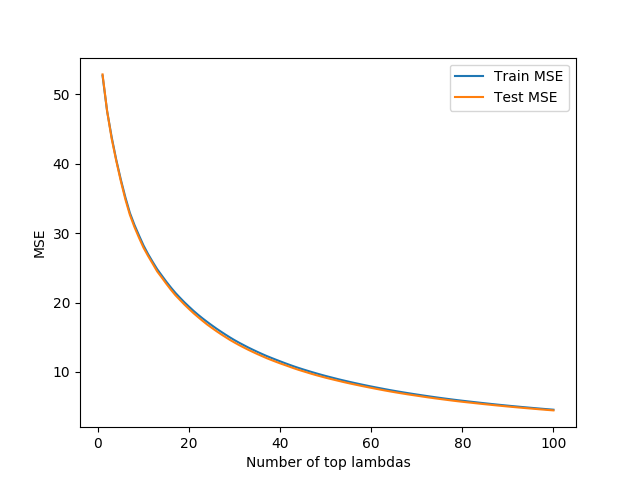
\includegraphics[width=9cm, height=6cm]{plots/A6c_1.png} \newline

For fractional error: \\
For k = 1 to 100, d = 784,  plot $1 - \frac{\sum_{i=1}^{k} \lambda_i}{\sum_{i=1}^{d} \lambda_i}$ \\
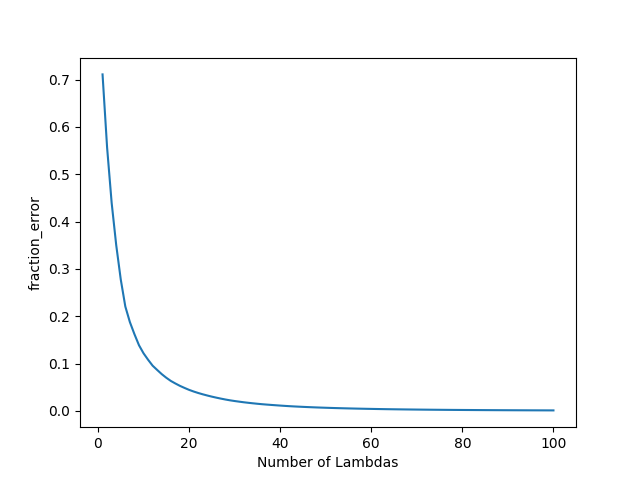
\includegraphics[width=9cm, height=6cm]{plots/A6c_2.png} \newline

\begin{minted}[mathescape,linenos,obeytabs=true,tabsize=2]{python}
# plot mse
mean_squared_error_list_train = []
mean_squared_error_list_test = []
for k in range(0, 100):
	print("K: ", k)
	reconstructed = np.dot(V[:k, :].T.dot(V[:k, :]), demean_X_train[:, :].T).T
	MSE_train = np.sum((reconstructed - demean_X_train) ** 2) / demean_X_train.shape[0]
	mean_squared_error_list_train.append(MSE_train)
	
	reconstructed_test = np.dot(V[:k, :].T.dot(V[:k, :]), demean_X_test[:, :].T).T
	MSE_test = np.sum((reconstructed_test - demean_X_test) ** 2) / demean_X_test.shape[0]
	mean_squared_error_list_test.append(MSE_test)

plt.plot(range(1, 101), mean_squared_error_list_train, label="Train MSE")
plt.plot(range(1, 101), mean_squared_error_list_test, label="Test MSE")
plt.xlabel("Number of top lambdas")
plt.ylabel("MSE")
plt.legend()
plt.savefig("/Users/yinruideng/Desktop/senior_spring/cse546/hw/hw3/latex/plots/A6c_1.png")
plt.show()


# plot construction error
eigenvalues_sum = sum(eigenvalues)
fraction_error_list = []
for k in range(0,100):
	fraction_error = 1 - np.sum(eigenvalues[:(k+1)]) / eigenvalues_sum
	fraction_error_list.append(fraction_error)

plt.plot(range(1, 101), fraction_error_list)
plt.xlabel("Number of Lambdas")
plt.ylabel("fraction_error")
plt.savefig("/Users/yinruideng/Desktop/senior_spring/cse546/hw/hw3/latex/plots/A6c_2.png")
plt.show()
\end{minted}

\subsection*{d.}

\fcolorbox{red}{white}{ Solution:} \\
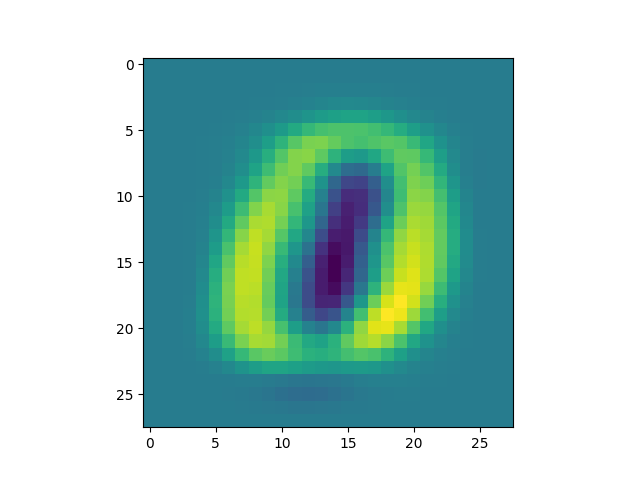
\includegraphics[width=3cm, height=2cm]{plots/A6d/A6d_0.png}
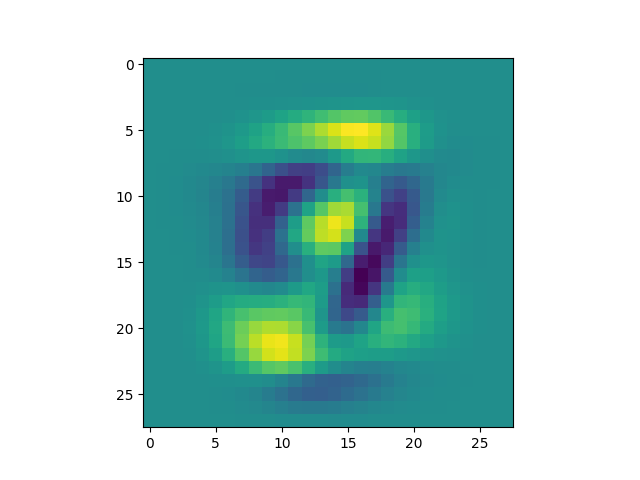
\includegraphics[width=3cm, height=2cm]{plots/A6d/A6d_1.png}
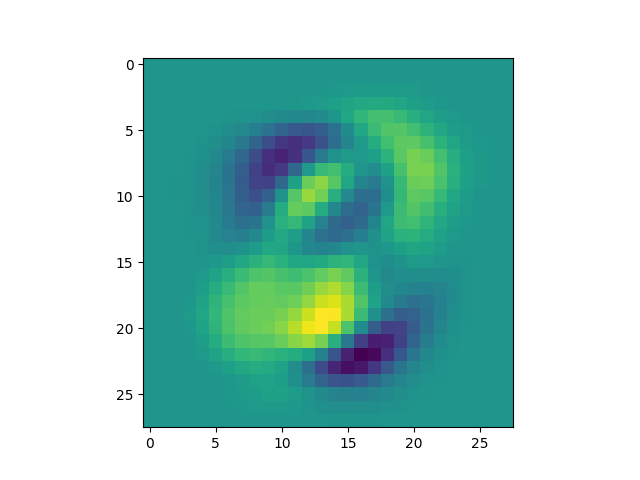
\includegraphics[width=3cm, height=2cm]{plots/A6d/A6d_2.png}
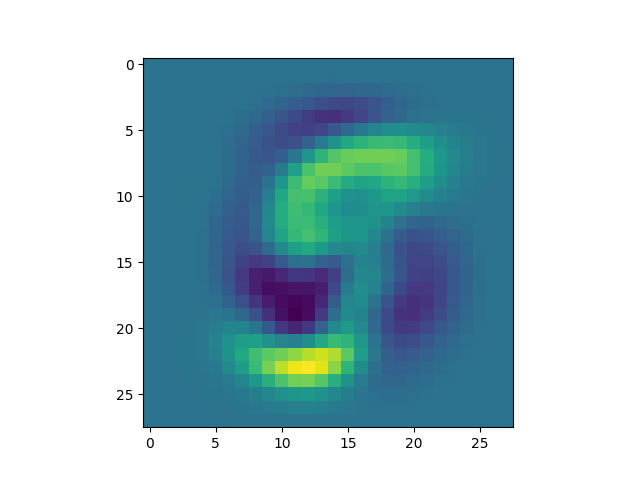
\includegraphics[width=3cm, height=2cm]{plots/A6d/A6d_3.png}
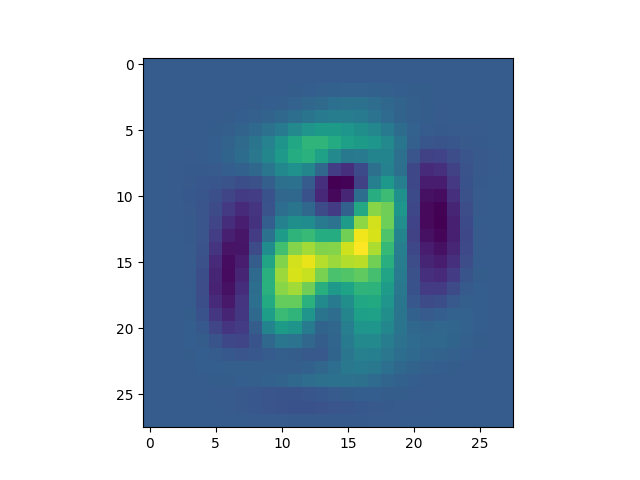
\includegraphics[width=3cm, height=2cm]{plots/A6d/A6d_4.png}
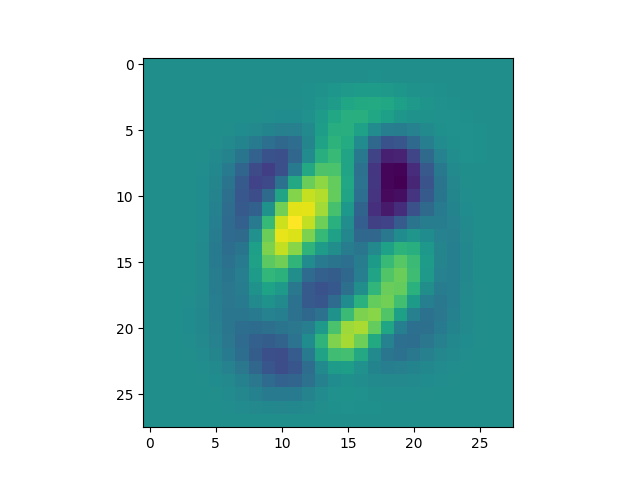
\includegraphics[width=3cm, height=2cm]{plots/A6d/A6d_5.png}
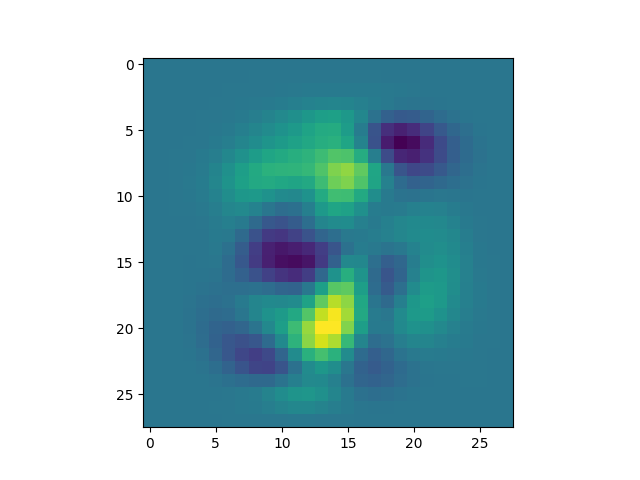
\includegraphics[width=3cm, height=2cm]{plots/A6d/A6d_6.png}
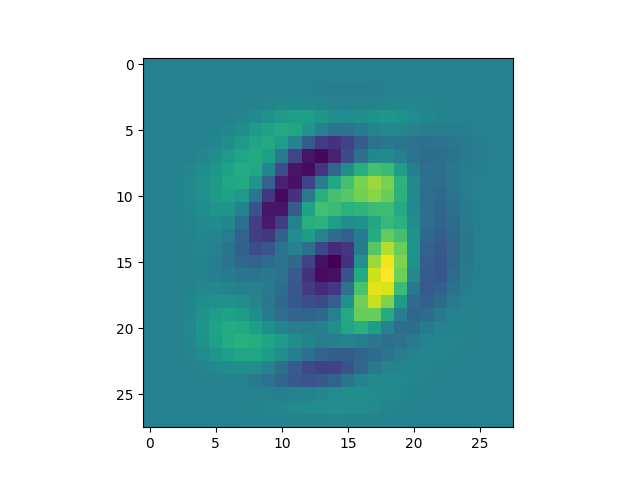
\includegraphics[width=3cm, height=2cm]{plots/A6d/A6d_7.png}
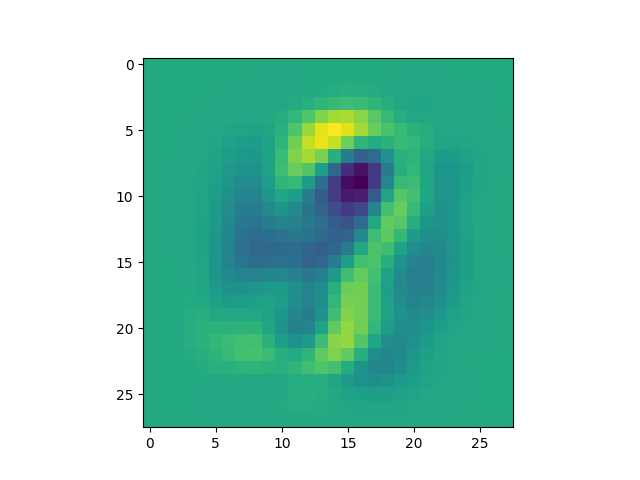
\includegraphics[width=3cm, height=2cm]{plots/A6d/A6d_8.png}
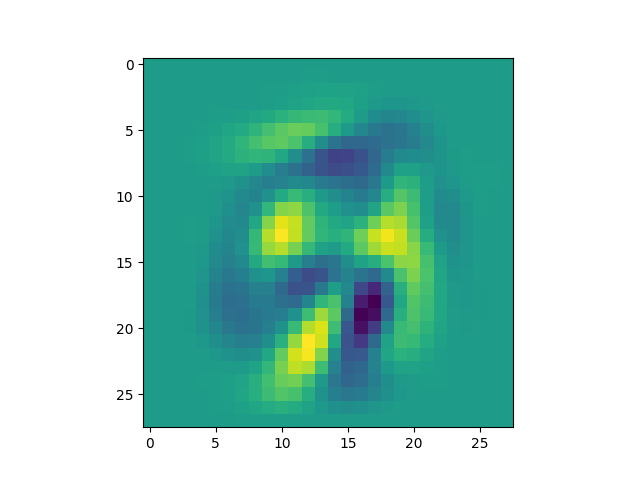
\includegraphics[width=3cm, height=2cm]{plots/A6d/A6d_9.png} \\

Interpretation: \\
Each of the image represent a PCA direction. It is a feature space with the highest variation. We can capture most of the variation and information through the top directions and thus we can reconstruct fairly close data. 

\begin{minted}[mathescape,linenos,obeytabs=true,tabsize=2]{python}
# ========================= A6d =========================
for k in range(10):
	plt.imshow(V[k,:].reshape((28,28)))
	plt.savefig("/Users/yinruideng/Desktop/senior_spring/cse546/hw/hw3/latex/plots/A6d/A6d_"+
						str(k)+".png")
	plt.show()

\end{minted}
\subsection*{e.}
\fcolorbox{red}{white}{ Solution:} \\
Plot the comparison between different number of top eigenvalues for [5, 15, 40, 100]:\\
For y = 2: \\
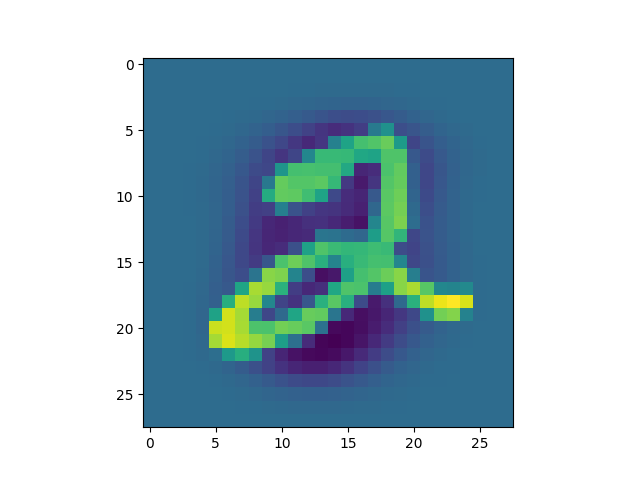
\includegraphics[width=3cm, height=2cm]{plots/A6e/A6e_5.png}
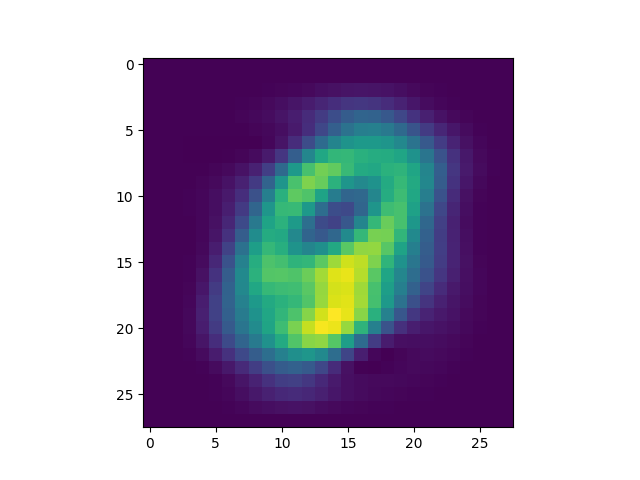
\includegraphics[width=3cm, height=2cm]{plots/A6e/A6e_5_5.png}
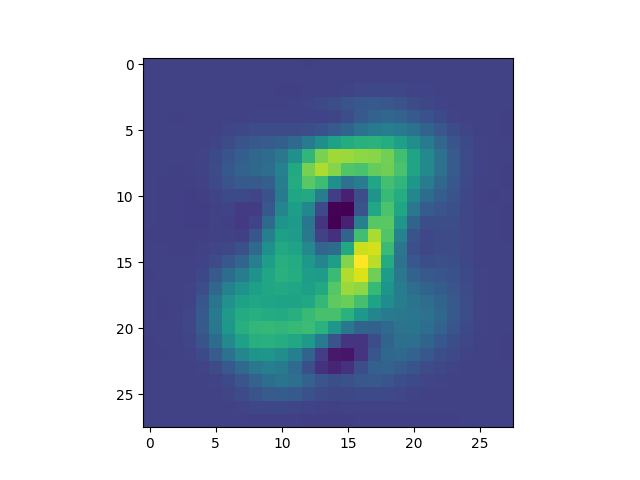
\includegraphics[width=3cm, height=2cm]{plots/A6e/A6e_5_15.png}
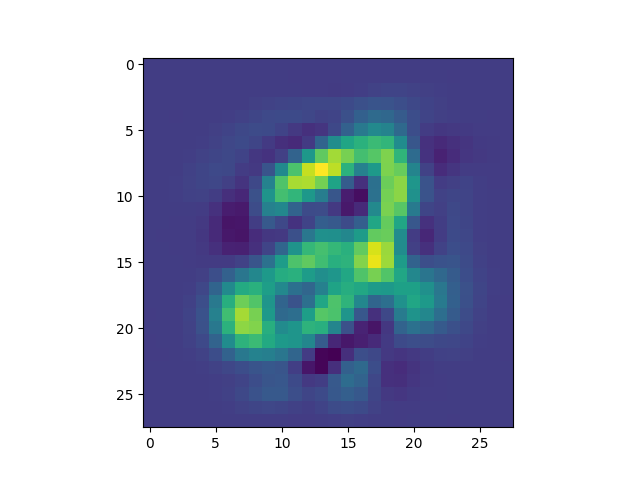
\includegraphics[width=3cm, height=2cm]{plots/A6e/A6e_5_40.png}
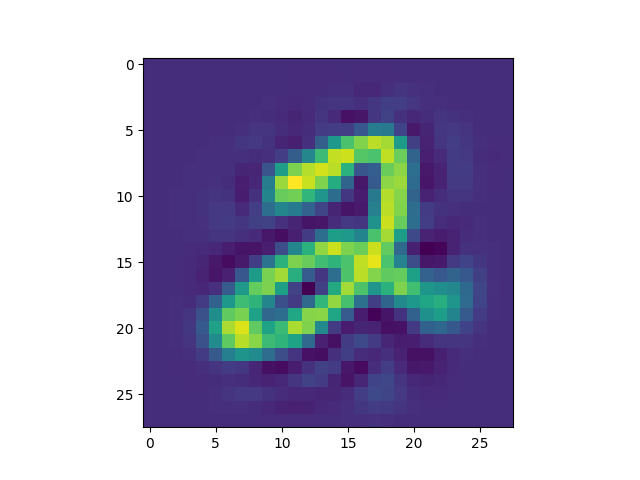
\includegraphics[width=3cm, height=2cm]{plots/A6e/A6e_5_100.png} \\
For y = 6: \\
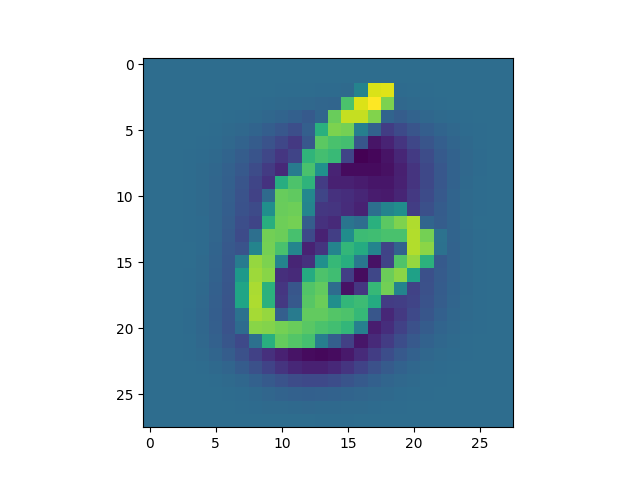
\includegraphics[width=3cm, height=2cm]{plots/A6e/A6e_13.png}
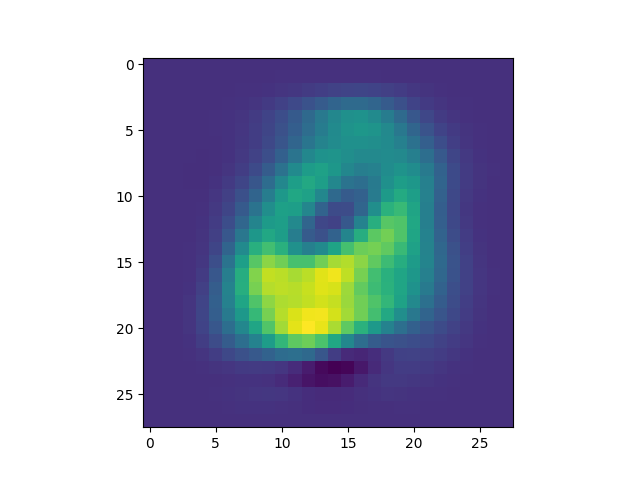
\includegraphics[width=3cm, height=2cm]{plots/A6e/A6e_13_5.png}
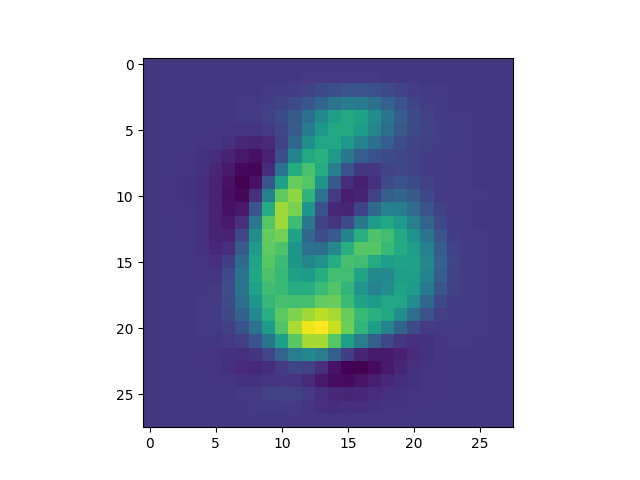
\includegraphics[width=3cm, height=2cm]{plots/A6e/A6e_13_15.png}
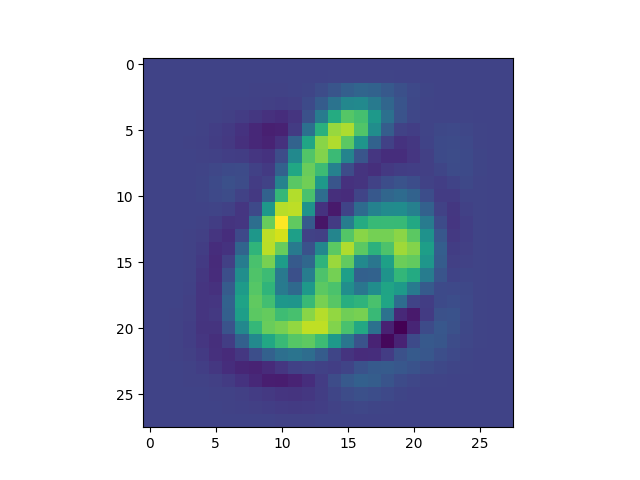
\includegraphics[width=3cm, height=2cm]{plots/A6e/A6e_13_40.png}
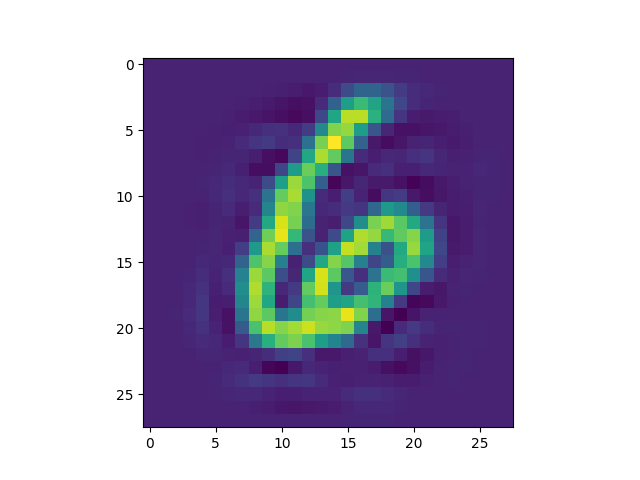
\includegraphics[width=3cm, height=2cm]{plots/A6e/A6e_13_100.png} \\
For y = 7: \\
\includegraphics[width=3cm, height=2cm]{plots/A6e/A6e_15.png}
\includegraphics[width=3cm, height=2cm]{plots/A6e/A6e_15_5.png}
\includegraphics[width=3cm, height=2cm]{plots/A6e/A6e_15_15.png}
\includegraphics[width=3cm, height=2cm]{plots/A6e/A6e_15_40.png}
\includegraphics[width=3cm, height=2cm]{plots/A6e/A6e_15_100.png} \\

Interpretation: \\
For this reconstruction process, we used 5, 15, 40, 100 top lambdas to reconstruct the image, and we can see that with more dimensionality we got better representation of the original image. So basically, more dimensionality we used, we could capture more variation in the data.







\begin{minted}[mathescape,linenos,obeytabs=true,tabsize=2]{python}
# ========================= A6e =========================
y_train[5] # =2
y_train[13] # =6
y_train[15] # =7

for y in [5, 13, 15]:  # this is the index of y in the X_train
	plt.imshow(X_train[y,:].reshape((28,28)))
	plt.savefig("/Users/yinruideng/Desktop/senior_spring/cse546/hw/hw3/latex/plots/A6e/A6e_"+
	str(y)+".png")
	plt.show()
	
	for k in [5, 15, 40, 100]:
		plt.imshow(np.dot(V[:k, :].T.dot(V[:k, :]), X_train[:, :].T).T[y].reshape((28, 28)))
		plt.savefig("/Users/yinruideng/Desktop/senior_spring/cse546/hw/hw3/latex/plots/A6e/A6e_" + 
		str(y) + "_"+str(k)+".png")
		plt.show()

# test case
plt.imshow(np.dot(V[:k, :].T.dot(V[:k, :]), X_train[:, :].T).T[y].reshape((28, 28)))
plt.show()
\end{minted}

















\end{document}